\documentclass[letter, 10pt]{article}
\usepackage[utf8]{inputenc}
\usepackage[spanish]{babel}
\usepackage{amsfonts}
\usepackage{amsmath}
\usepackage[dvips]{graphicx}
\usepackage{url}
\usepackage[top=3cm,bottom=3cm,left=3.5cm,right=3.5cm,footskip=1.5cm,headheight=1.5cm,headsep=.5cm,textheight=3cm]{geometry}
\usepackage[linesnumbered, boxruled]{algorithm2e}
%%\usepackage[]{algorithm}

\begin{document}
\title{Inteligencia Artificial \\ \begin{Large}Informe Final: Problema alanced Academic Curriculum Problem\end{Large}}
\author{[Nombre autor]}
\date{\today}
\maketitle


%--------------------No borrar esta secci\'on--------------------------------%
\section*{Evaluación}

\begin{tabular}{ll}
Mejoras 1ra Entrega (10 \%): &  \underline{\hspace{2cm}}\\
Codigo Fuente (10 \%): &  \underline{\hspace{2cm}}\\
Representación (15 \%):  & \underline{\hspace{2cm}} \\
Descripción del algoritmo (20 \%):  & \underline{\hspace{2cm}} \\
Experimentos (10 \%):  & \underline{\hspace{2cm}} \\
Resultados (10 \%):  & \underline{\hspace{2cm}} \\
Conclusiones (20 \%): &  \underline{\hspace{2cm}}\\
Bibliografía (5 \%): & \underline{\hspace{2cm}}\\
 &  \\
\textbf{Nota Final (100)}:   & \underline{\hspace{2cm}}
\end{tabular}
%---------------------------------------------------------------------------%

\begin{abstract}
Resumen del informe en no m\'as de 10 l\'ineas.
\end{abstract}

\section{Introducción}

\section{Definición del Problema}

\section{Estado del Arte}

\section{Modelo Matemático}


\section{Representación}
\subsection{Cromosoma}
En la búsqueda de una solución a este problema, se implementó un Algoritmo
Genético cuyo cromosoma corresponde a un arreglo de números enteros. El
cromosoma tiene, entonces, la siguiente forma:

$$
	[x_{1},x_{2}, \dots ,x_{n-1},x_{n}]
$$

En esta representación la posición $i$ del arreglo representa al ramo $x_{i}$
del plan académico. El dominio de cada curso $x_{i}$ sera un conjunto de enteros
que van desde 1 hasta el número de periodos que debe contemplar la malla
curricular. En otras palabras, cada valor del arreglo indicara el semestre en el
cual se dictará el curso $x_{i}$.

Ejemplificando lo anterior para 

\subsubsection{Ventajas de la representación}
Entre las ventajas de esta representación destacan:
\begin{itemize}
	\item El bajo costo de traducción entre la representación y la solución
          en lenguaje natural.
	\item Manejar de forma simple la restricción dura: "Todos los ramos
          deben ser instanciado una sola vez", del modelo matemático.
	\item Facilitar el calculo del cumplimiento y violación de las
          restricciones blandas relacionadas con: los pre-requisitos, créditos y
          numero de ramos máximos y mínimos.
\end{itemize}

\subsubsection{Desventajas de la representación}
\begin{itemize}
	\item Por si sola, esta representación, es extremadamente sensible a
          operadores genéticos simples de mutación o cruzamiento, por lo que no
          es capaz de conservar o xxx las restricciones temporales de
          pre-requisitos.
\end{itemize}

\subsection{Representaciónes auxiliares}
\subsubsection{Esqueleto}
El estudio de este problema revela un alto grado de conexión entre ramos y el
periodo en el cual son instanciados heredado de las restricciones temporales de
los pre-requisitos. Lo anterior inspiro la creación de una representación
auxiliar, propia de cada problema, que fue llamada "esqueleto" del problema.
Este ``esqueleto'' corresponde a un arreglo binario donde el curso $x_{i}$ tendrá
el valor 1 si es parte de algún árbol de pre-requisitos y 0 si no lo es. De esta
manera el arreglo ``esqueleto'' es una representación directa de los grafos de
restricciones y servirá para crear, de forma primitiva, mejoras a los operadores
genéticos en busca de una minimización en la tasa de violación de restricciones
blandas referentes a los pre-requisitos.

\subsubsection{Max Period}
Para tratar otras las restricciones nacidas de los pre-requisitos, se utilizó un
arreglo de enteros el cual indicaba el resultado de calcular el máximo periodo
en el cual un ramo puede ser instanciado. Pasado este periodo la instancicion de
dicho ramo generará irremediablemente soluciones infactibles. Al igual que la
representación esqueleto, "max period" es una representación propia de cada
problema y no de cada solución.

\subsubsection{Otras representaciones}
\begin{description}
\item[Pre-requisitos:] Los pre-requisitos fueron representados con una matrix
  bidimencional con columnas de largo variable, donde cada columna representa un
  arreglo entero con el identificador del curso requisito.
\item[Creditos:] Arreglo entero que indica el crédito de cada curso.
\item[Cursos:] Arreglo de string que contiene el nombre de cada curso.

\end{description}


\section{Descripción del algoritmo}
Como se mencionó en la sección anterior, se desarrolló un Algoritmo Genético
para buscar mallas curriculares balanceadas.  La implementación de este tipo de
meta-heristicas requiere el diseño de procedimientos para la creación de una
población inicial, calculo de la calidad de la solución, procedimientos de
operadores de mutación, cruzamiento y elitismo, de procedimientos de evaluación
de soluciones, de una rutina para la selección de individuos, y el
establecimiento de parámetros propios como el tamaño de la población y el número
de generaciones.  A continuación se detallan algunos de estos elementos.

\subsection{Generación de la población inicial}
Debido al número y grado de conexión entre los cursos y los periodos con las
restricciones, se decidió generar soluciones aleatorias que cumplieran con toda
y cada una de las restricciones del problema. Es decir, cada individuo cumplirá
no solo con el mínimo y máximo numero de créditos y ramos por semestre, si no
que también asegurará que los pre-requisitos de cada ramo sean instanciados con
anterioridad. Esto ultimo se logró filtrando de forma dinámica, en cada periodo,
los ramos potencialmente instanciables, para luego seleccionar al azar uno de
ellos. En este proceso la representación "Max Period" juego un papel importante
indicando tempranamente soluciones infactibles en las cuales no sería posible
colocar todos los ramos dentro de una malla. Las soluciones que no lograron
alcanzar el nivel de factibilidad óptimo, fueron descartadas. Para las
instancias analizadas este procedimiento demostró ser eficiente manteniendo el
nivel de soluciones no factibles a niveles bajos. El algoritmo ~\ref{alg:gennew}
presenta el pseudo código de esta rutina.

\begin{algorithm}[H]
\SetLine
\KwIn{bacp 8, 10 o 12 de csplib}
\KwOut{Cromosoma de una solución}
\While{Quedan ramos por instanciar}{
Calcular cantidad ramos por instanciar\;
\ForEach{Periodo $p$}{
Crear vector vacío $ramosCandidatos$ \;
\ForEach{Ramo $r$}{
\If{Ramo $r$ tiene todos los requisitos instanciados}{
$ramosCandidatos$ $\gets$ $r$ \;
}
}
\If{$ramosCandidatos$ != $\emptyset$}{
Elegir ramo $i \in ramosCandidatos$ al azar \;
\If{ramo $i$ en el periodo $p$ no rompe restricciones}
{
\tcc{Esta verificación incluye el asegurarse que todos los periodos cuentan con el mínimo de ramos y créditos esperados, antes de tratar de alcanzar el máximo.}
$Cromosoma[i] = p$
}
}
}
\If{no se instanciaron nuevos ramos}{
Detener y desechar solución\;
}
}
\caption{Generar soluciones}
\label{alg:gennew}
\end{algorithm}

\subsection{Calculo de la calidad de la solución}
Siguiendo el modelo matemático presentado en la sección 4, la calidad de la
solución viene dada por la suma de las desviaciones a la media.  A esta
desviación se le suman el numero de restricciones violadas por la solución. Una
solución de mayor calidad, sera aquella que posea un menor valor de esta
sumatoria. El algoritmo ~\ref{alg:fit} muestra el pseudocódigo que permite
calcular este valor.

\begin{algorithm}[H]
\SetLine
\KwIn{Solución $S$, numero de periodos $P$, sumatoria de créditos de todos los ramos $C$}
\KwOut{Fitness $f$}
$w \gets \frac{C}{P}$
\tcc{Promedio de esperado de créditos por semestre que representa el máximo balance teorico}

$f \gets 0$ \;
\ForEach{Periodo $i$}{
$p_{i} \gets$ calculo de los créditos en periodo $i$ según $S$ \;
$f \gets f + |w - p_{i}|$ \;
}
$g \gets$ número de restricciones insatisfechas \;
$f \gets f * (1+g)$ \;

\KwResult{$f$}

\caption{Fitness}
\label{alg:fit}
\end{algorithm}


\subsection{Operador: Mutación}
El operador unario de mutación consiste en seleccionar un individuo y mover
algunos de sus ramos a otro semestre.  Esta rutina afecta a todos los ramos y es
gatillada previa evaluación de la tasa de aceptación de mutación.
Adicionalmente se diseñaron características combinables para este operador los
cuales buscaban interactuar con las restricciones en distintos grados:

\begin{description}
\item[Mutación normal:] Que evalua las restricciones de mínimos y
  máximos créditos antes de operar.
\item[Mutación ciega: ] La cual no tiene en cuenta las restricciones de
  mínimos y máximos créditos antes de operar
\item[Mutación con primera mejora:] La cual intenta operar un
  determinado numero de veces buscando una mejora en la solución.
\item[Mutación con esqueleto:] Que opera solo si el ramo no es parte del
  esqueleto de la solución.
\end{description}

El algoritmo ~\ref{alg:mut} muestra la versión combinada de todas las
características antes mencionadas.


\begin{algorithm}[H]
\SetLine
\KwIn{Solución $S$, tasa de mutación $M$, esqueleto $E$, intentos $I$}
\KwOut{Cromosoma de una solución}
$p \gets$ número al azar entre 0 y 1 \;
\If{$p \leq M$}{
\
\ForEach{Ramo $i$}{
\If{$i \in E$}{
Ignorar y continuar iteración \;
}
\If{$p \leq M$}{
$j \gets$ periodo al azar;

\If{Si el periodo $j$ no esta excedido en créditos}{
$S.Cromosoma[i] = j$ \;
}
\If{Solución no ha mejorado en los últimos $I$ intentos}{
$i--$
}
}
}
\KwResult{Cromosoma de la solución S}
}

\caption{Operador: mutación}
\label{alg:mut}
\end{algorithm}


\subsection{Operador: Cruzamiento}
El operador se define como cruzamiento en un punto del cromosoma. Se crearon dos
versiones:
\begin{description}
\item[Cruzamiento en un punto de ramos:] Aplica el cruzamiento directamente al
  cromosoma.
\item[Cruzamiento en un punto de periodos:] Calcula los ramos de cada periodo e
  intenta intercambiar semestres completos entre las dos soluciones.
\end{description}

Al igual que la mutación, el cruzamiento posee una variante que toma en cuenta
los ramos que pertenecen al esqueleto de la solución.  Dada la gran diferencia
entre cada implementación, el algoritmo ~\ref{alg:cruz} solo muestra el
pseudocódigo del cruzamiento de semestres enteros.

\begin{algorithm}[H]
\SetLine
\KwIn{Soluciones $S_{1},S_{2}$, tasa de cruzamiento $C$, esqueleto $E$}
\KwOut{Cromosomas de $Z_{1}$ y $Z_{2}$ de dos soluciones}
$w \gets$ número al azar entre 0 y 1 \;
\If{$w \leq C$}{
$Z_{1} = S_{1}$ \;
$Z_{2} = S_{2}$ \;
periodo $P \gets$ periodo al azar distinto del primer y último periodo \;

\ForEach{Ramo $i$}{
\If{$i \in E$}{
Ignorar y continuar \;
}
\If{$S_{1}.Cromosoma[i] \geq P$ o $S_{2}.Cromosoma[i] \geq P$}{
	$Z_{2}.Cromosoma[i] = S_{1}.Cromosoma[i]$ \; 
	$Z_{1}.Cromosoma[i] = S_{2}.Cromosoma[i]$ \;
}
}
\KwResult{$Z_{1},Z_{2}$}
}

\caption{Operador: Cruzamiento de semestres en un punto}
\label{alg:cruz}
\end{algorithm}

\subsection{Elitismo}
Se utilizo un operador elitismo estándar de tamaño 1. Es decir, seleccionar el
mejor elemento de una población y traspasarlo directamente a la siguiente.  El
algoritmo ~\ref{alg:elite} muestra la rutina de este procedimiento.

\begin{algorithm}[H]
\SetLine
\KwIn{Población actual $P$, Población siguiente $O$}

$S \gets$ mejor solución de la población $P$ \;
$O \gets \{S\}$ \;

\caption{Operador: Elitismo}
\label{alg:elite}
\end{algorithm}

\subsection{Algoritmo Genético}
El algoritmo genético se ejecutó con tres pequeñas diferencias: Con elitismo,
sin elitismo y con restart en el elitismo.  El motivo de estos cambios se
explicara en la siguiente sección ~\ref{experimentos}. El algoritmo
~\ref{alg:genetico} presenta la rutina de ejecución del método desarrollado.

\begin{algorithm}[H]
\SetLine
\KwIn{generaciones $G$, tamaño de la población $T$, tasa de mutación $M$, tasa de cruzamiento $C$}

Generar población inicial $P_{a}$ \;
Crear población siguientes $P_{b} \gets \emptyset$ \;
Calcular calidad de soluciones de $P_{a}$ \;
\While{no se hayan alcanzado el numero de generaciones $G$}{
\If{se debe aplicar elitismo}{
Operador Elitismo con $P_{a}$ y $P_{b}$ \;
}
\While{$P_{b}$ no tenga el tamaño de población $T$}{
Operador Mutación\;

Operador Cruzamiento\;
}
$P_{a} \gets P_{b}$ \;
Calcular calidad de soluciones de $P_{a}$ \;
$P_{b} \gets \emptyset$ \;
}
\caption{Algoritmo Génetico}
\label{alg:genetico}
\end{algorithm}

\section{Implemetación}
Para implementar el algoritmo se desarrollo un software en C++ utilizando un
paradigma orientado a objetos. El codigo de esta implementación se encuentra
disponible en un repositorio GIT en
GitHub \footnote{https://github.com/Aierk/bacp\_ga\_eclipse}. La imagen
~\ref{clases} presenta el diagrama, resumido, de clases de la implementación.

\begin{figure}[h!]
  \centering
  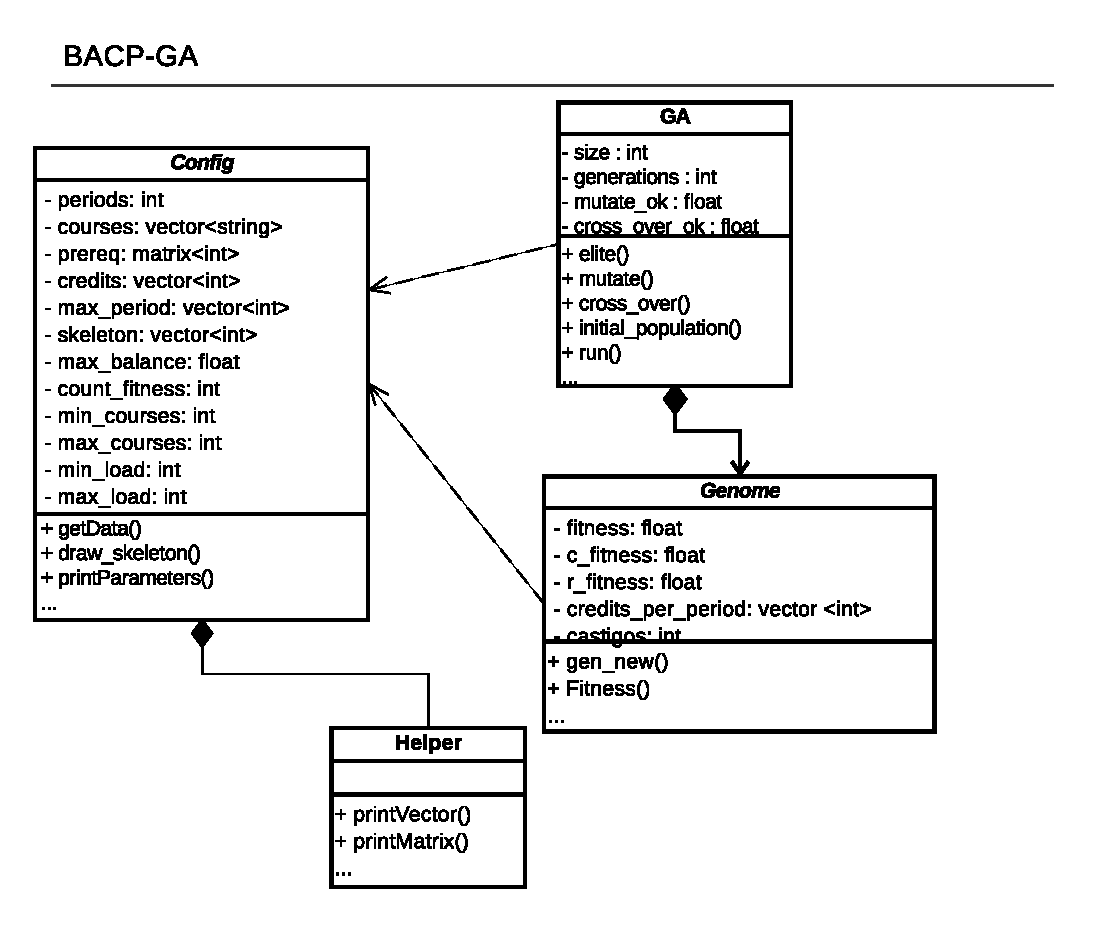
\includegraphics[width=0.7\textwidth]{ga}
  \caption{Diagrama de clases}
\end{figure}

\section{Experimentos}
\label{experimentos}
Al igual que en los papers referenciados en la sección Estado del Arte, los
experimentos se realizaron utilizando los casos oficiales almacenados en CSPLib
para mallas de 8, 10 y 12 periodos. A continuación se listaran los experimentos
de forma cualitativa:

\subsection{Determinación de la población y generación}
Estos experimentos tenian como tenian como objetivo observar el comportamiento
del algoritmo con generaciones cercanas a 100 y poblaciónes del ordenes muy
menores a ellas.  Utilizando los operadores mutación y cruzamiento sin mejoras,
se observo que el algoritmo convergia muy rapido y no lograba mejorar
considerablemente la población inicial. Estos experimentos tambien arrojaron que
los castigos de la función Fitness, utilizada para evaluar las soluciones, no
penalizaban los suficiente a las soluciones infactibles. Una vez terminados
estos experimentos se genero una nueva función Fitness que castigaba de manera
mas acertada las soluciones infactibles y que poblaciones de 30 individuos en
100 generaciones permitia a las soluciones evolucionar de manera adecuada.

\subsection{Determinación de las probabilidades de mutación y cruzamiento}
Durante los experimentos se observó que la tasa de mejora que aplicaban los
operadores cruzammiento y mutación era extremadamente baja. Analizando la
evolución de los individuos se noto que empeoraban de forma muy rapida
especialmente al utilizar al aumentar la probabilidad operador de mutación,
apareciendo peridos sin ramos o con la mayoria de los requerimientos rotos.
Esto ayudo a crear versiones mejoradas de ambos operados (presentados en la
sección anterior) que demostraron dismuir la desviación de las nuevas
poblaciones y de mejorar considerablemente y rapidamente a la población inicial.

\subsection{Importancia Elitismo}
Como se aprecio en los experimentos antes mecionados, y debido al alto grado de
conectividad entre los ramos y las restricciones, las poblaciones tienden a
empeorar, por lo que el uso de elitismo es critico en la obtención de un resultado optimo.

\begin{center}
% GNUPLOT: LaTeX picture
\setlength{\unitlength}{0.240900pt}
\ifx\plotpoint\undefined\newsavebox{\plotpoint}\fi
\sbox{\plotpoint}{\rule[-0.200pt]{0.400pt}{0.400pt}}%
\begin{picture}(1500,900)(0,0)
\sbox{\plotpoint}{\rule[-0.200pt]{0.400pt}{0.400pt}}%
\put(110.0,131.0){\rule[-0.200pt]{4.818pt}{0.400pt}}
\put(90,131){\makebox(0,0)[r]{ 0}}
\put(1419.0,131.0){\rule[-0.200pt]{4.818pt}{0.400pt}}
\put(110.0,196.0){\rule[-0.200pt]{4.818pt}{0.400pt}}
\put(90,196){\makebox(0,0)[r]{ 2}}
\put(1419.0,196.0){\rule[-0.200pt]{4.818pt}{0.400pt}}
\put(110.0,260.0){\rule[-0.200pt]{4.818pt}{0.400pt}}
\put(90,260){\makebox(0,0)[r]{ 4}}
\put(1419.0,260.0){\rule[-0.200pt]{4.818pt}{0.400pt}}
\put(110.0,325.0){\rule[-0.200pt]{4.818pt}{0.400pt}}
\put(90,325){\makebox(0,0)[r]{ 6}}
\put(1419.0,325.0){\rule[-0.200pt]{4.818pt}{0.400pt}}
\put(110.0,389.0){\rule[-0.200pt]{4.818pt}{0.400pt}}
\put(90,389){\makebox(0,0)[r]{ 8}}
\put(1419.0,389.0){\rule[-0.200pt]{4.818pt}{0.400pt}}
\put(110.0,454.0){\rule[-0.200pt]{4.818pt}{0.400pt}}
\put(90,454){\makebox(0,0)[r]{ 10}}
\put(1419.0,454.0){\rule[-0.200pt]{4.818pt}{0.400pt}}
\put(110.0,518.0){\rule[-0.200pt]{4.818pt}{0.400pt}}
\put(90,518){\makebox(0,0)[r]{ 12}}
\put(1419.0,518.0){\rule[-0.200pt]{4.818pt}{0.400pt}}
\put(110.0,583.0){\rule[-0.200pt]{4.818pt}{0.400pt}}
\put(90,583){\makebox(0,0)[r]{ 14}}
\put(1419.0,583.0){\rule[-0.200pt]{4.818pt}{0.400pt}}
\put(110.0,647.0){\rule[-0.200pt]{4.818pt}{0.400pt}}
\put(90,647){\makebox(0,0)[r]{ 16}}
\put(1419.0,647.0){\rule[-0.200pt]{4.818pt}{0.400pt}}
\put(110.0,712.0){\rule[-0.200pt]{4.818pt}{0.400pt}}
\put(90,712){\makebox(0,0)[r]{ 18}}
\put(1419.0,712.0){\rule[-0.200pt]{4.818pt}{0.400pt}}
\put(110.0,776.0){\rule[-0.200pt]{4.818pt}{0.400pt}}
\put(90,776){\makebox(0,0)[r]{ 20}}
\put(1419.0,776.0){\rule[-0.200pt]{4.818pt}{0.400pt}}
\put(110.0,131.0){\rule[-0.200pt]{0.400pt}{4.818pt}}
\put(110,90){\makebox(0,0){ 0}}
\put(110.0,756.0){\rule[-0.200pt]{0.400pt}{4.818pt}}
\put(243.0,131.0){\rule[-0.200pt]{0.400pt}{4.818pt}}
\put(243,90){\makebox(0,0){ 10}}
\put(243.0,756.0){\rule[-0.200pt]{0.400pt}{4.818pt}}
\put(376.0,131.0){\rule[-0.200pt]{0.400pt}{4.818pt}}
\put(376,90){\makebox(0,0){ 20}}
\put(376.0,756.0){\rule[-0.200pt]{0.400pt}{4.818pt}}
\put(509.0,131.0){\rule[-0.200pt]{0.400pt}{4.818pt}}
\put(509,90){\makebox(0,0){ 30}}
\put(509.0,756.0){\rule[-0.200pt]{0.400pt}{4.818pt}}
\put(642.0,131.0){\rule[-0.200pt]{0.400pt}{4.818pt}}
\put(642,90){\makebox(0,0){ 40}}
\put(642.0,756.0){\rule[-0.200pt]{0.400pt}{4.818pt}}
\put(774.0,131.0){\rule[-0.200pt]{0.400pt}{4.818pt}}
\put(774,90){\makebox(0,0){ 50}}
\put(774.0,756.0){\rule[-0.200pt]{0.400pt}{4.818pt}}
\put(907.0,131.0){\rule[-0.200pt]{0.400pt}{4.818pt}}
\put(907,90){\makebox(0,0){ 60}}
\put(907.0,756.0){\rule[-0.200pt]{0.400pt}{4.818pt}}
\put(1040.0,131.0){\rule[-0.200pt]{0.400pt}{4.818pt}}
\put(1040,90){\makebox(0,0){ 70}}
\put(1040.0,756.0){\rule[-0.200pt]{0.400pt}{4.818pt}}
\put(1173.0,131.0){\rule[-0.200pt]{0.400pt}{4.818pt}}
\put(1173,90){\makebox(0,0){ 80}}
\put(1173.0,756.0){\rule[-0.200pt]{0.400pt}{4.818pt}}
\put(1306.0,131.0){\rule[-0.200pt]{0.400pt}{4.818pt}}
\put(1306,90){\makebox(0,0){ 90}}
\put(1306.0,756.0){\rule[-0.200pt]{0.400pt}{4.818pt}}
\put(1439.0,131.0){\rule[-0.200pt]{0.400pt}{4.818pt}}
\put(1439,90){\makebox(0,0){ 100}}
\put(1439.0,756.0){\rule[-0.200pt]{0.400pt}{4.818pt}}
\put(110.0,131.0){\rule[-0.200pt]{0.400pt}{155.380pt}}
\put(110.0,131.0){\rule[-0.200pt]{320.156pt}{0.400pt}}
\put(1439.0,131.0){\rule[-0.200pt]{0.400pt}{155.380pt}}
\put(110.0,776.0){\rule[-0.200pt]{320.156pt}{0.400pt}}
\put(774,29){\makebox(0,0){Generaciones}}
\put(774,838){\makebox(0,0){BACP 8 - Mut. y Cruz. Simple con elitismo}}
\sbox{\plotpoint}{\rule[-0.400pt]{0.800pt}{0.800pt}}%
\sbox{\plotpoint}{\rule[-0.200pt]{0.400pt}{0.400pt}}%
\put(1279,736){\makebox(0,0)[r]{Mejor}}
\sbox{\plotpoint}{\rule[-0.400pt]{0.800pt}{0.800pt}}%
\put(1299.0,736.0){\rule[-0.400pt]{24.090pt}{0.800pt}}
\put(123,534){\usebox{\plotpoint}}
\multiput(377.41,527.04)(0.509,-0.947){19}{\rule{0.123pt}{1.677pt}}
\multiput(374.34,530.52)(13.000,-20.519){2}{\rule{0.800pt}{0.838pt}}
\put(123.0,534.0){\rule[-0.400pt]{60.948pt}{0.800pt}}
\multiput(1121.41,492.57)(0.509,-2.643){19}{\rule{0.123pt}{4.200pt}}
\multiput(1118.34,501.28)(13.000,-56.283){2}{\rule{0.800pt}{2.100pt}}
\put(389.0,510.0){\rule[-0.400pt]{176.098pt}{0.800pt}}
\multiput(1307.41,411.22)(0.509,-5.290){19}{\rule{0.123pt}{8.138pt}}
\multiput(1304.34,428.11)(13.000,-112.108){2}{\rule{0.800pt}{4.069pt}}
\put(1133.0,445.0){\rule[-0.400pt]{41.676pt}{0.800pt}}
\put(1319.0,316.0){\rule[-0.400pt]{28.908pt}{0.800pt}}
\sbox{\plotpoint}{\rule[-0.200pt]{0.400pt}{0.400pt}}%
\put(1279,695){\makebox(0,0)[r]{Castigos}}
\put(1299.0,695.0){\rule[-0.200pt]{24.090pt}{0.400pt}}
\put(123,131){\usebox{\plotpoint}}
\put(123.0,131.0){\rule[-0.200pt]{317.024pt}{0.400pt}}
\put(1279,654){\makebox(0,0)[r]{Max. carga}}
\multiput(1299,654)(20.756,0.000){5}{\usebox{\plotpoint}}
\put(1399,654){\usebox{\plotpoint}}
\put(123,744){\usebox{\plotpoint}}
\put(123.00,744.00){\usebox{\plotpoint}}
\put(143.76,744.00){\usebox{\plotpoint}}
\put(164.51,744.00){\usebox{\plotpoint}}
\put(185.27,744.00){\usebox{\plotpoint}}
\put(206.02,744.00){\usebox{\plotpoint}}
\put(226.78,744.00){\usebox{\plotpoint}}
\put(247.53,744.00){\usebox{\plotpoint}}
\put(268.29,744.00){\usebox{\plotpoint}}
\put(289.04,744.00){\usebox{\plotpoint}}
\put(309.80,744.00){\usebox{\plotpoint}}
\put(330.56,744.00){\usebox{\plotpoint}}
\put(351.31,744.00){\usebox{\plotpoint}}
\put(372.07,744.00){\usebox{\plotpoint}}
\put(392.82,744.00){\usebox{\plotpoint}}
\put(413.58,744.00){\usebox{\plotpoint}}
\put(434.33,744.00){\usebox{\plotpoint}}
\put(455.09,744.00){\usebox{\plotpoint}}
\put(475.84,744.00){\usebox{\plotpoint}}
\put(496.60,744.00){\usebox{\plotpoint}}
\put(517.35,744.00){\usebox{\plotpoint}}
\put(538.11,744.00){\usebox{\plotpoint}}
\put(558.87,744.00){\usebox{\plotpoint}}
\put(579.62,744.00){\usebox{\plotpoint}}
\put(600.38,744.00){\usebox{\plotpoint}}
\put(621.13,744.00){\usebox{\plotpoint}}
\put(641.89,744.00){\usebox{\plotpoint}}
\put(662.64,744.00){\usebox{\plotpoint}}
\put(683.40,744.00){\usebox{\plotpoint}}
\put(704.15,744.00){\usebox{\plotpoint}}
\put(724.91,744.00){\usebox{\plotpoint}}
\put(745.66,744.00){\usebox{\plotpoint}}
\put(766.42,744.00){\usebox{\plotpoint}}
\put(787.18,744.00){\usebox{\plotpoint}}
\put(807.93,744.00){\usebox{\plotpoint}}
\put(828.69,744.00){\usebox{\plotpoint}}
\put(849.44,744.00){\usebox{\plotpoint}}
\put(870.20,744.00){\usebox{\plotpoint}}
\put(890.95,744.00){\usebox{\plotpoint}}
\put(911.71,744.00){\usebox{\plotpoint}}
\put(932.46,744.00){\usebox{\plotpoint}}
\put(953.22,744.00){\usebox{\plotpoint}}
\put(973.98,744.00){\usebox{\plotpoint}}
\put(994.73,744.00){\usebox{\plotpoint}}
\put(1015.49,744.00){\usebox{\plotpoint}}
\put(1036.24,744.00){\usebox{\plotpoint}}
\put(1057.00,744.00){\usebox{\plotpoint}}
\put(1077.75,744.00){\usebox{\plotpoint}}
\put(1098.51,744.00){\usebox{\plotpoint}}
\put(1119.26,744.00){\usebox{\plotpoint}}
\put(1140.02,744.00){\usebox{\plotpoint}}
\put(1160.77,744.00){\usebox{\plotpoint}}
\put(1181.53,744.00){\usebox{\plotpoint}}
\put(1202.29,744.00){\usebox{\plotpoint}}
\put(1223.04,744.00){\usebox{\plotpoint}}
\put(1243.80,744.00){\usebox{\plotpoint}}
\put(1264.55,744.00){\usebox{\plotpoint}}
\put(1285.31,744.00){\usebox{\plotpoint}}
\multiput(1306,744)(7.812,-19.229){2}{\usebox{\plotpoint}}
\put(1326.03,712.00){\usebox{\plotpoint}}
\put(1346.79,712.00){\usebox{\plotpoint}}
\put(1367.55,712.00){\usebox{\plotpoint}}
\put(1388.30,712.00){\usebox{\plotpoint}}
\put(1409.06,712.00){\usebox{\plotpoint}}
\put(1429.81,712.00){\usebox{\plotpoint}}
\put(1439,712){\usebox{\plotpoint}}
\put(110.0,131.0){\rule[-0.200pt]{0.400pt}{155.380pt}}
\put(110.0,131.0){\rule[-0.200pt]{320.156pt}{0.400pt}}
\put(1439.0,131.0){\rule[-0.200pt]{0.400pt}{155.380pt}}
\put(110.0,776.0){\rule[-0.200pt]{320.156pt}{0.400pt}}
\end{picture}

\end{center}




\begin{center}
% GNUPLOT: LaTeX picture
\setlength{\unitlength}{0.240900pt}
\ifx\plotpoint\undefined\newsavebox{\plotpoint}\fi
\sbox{\plotpoint}{\rule[-0.200pt]{0.400pt}{0.400pt}}%
\begin{picture}(1500,900)(0,0)
\sbox{\plotpoint}{\rule[-0.200pt]{0.400pt}{0.400pt}}%
\put(110.0,131.0){\rule[-0.200pt]{4.818pt}{0.400pt}}
\put(90,131){\makebox(0,0)[r]{ 0}}
\put(1419.0,131.0){\rule[-0.200pt]{4.818pt}{0.400pt}}
\put(110.0,239.0){\rule[-0.200pt]{4.818pt}{0.400pt}}
\put(90,239){\makebox(0,0)[r]{ 10}}
\put(1419.0,239.0){\rule[-0.200pt]{4.818pt}{0.400pt}}
\put(110.0,346.0){\rule[-0.200pt]{4.818pt}{0.400pt}}
\put(90,346){\makebox(0,0)[r]{ 20}}
\put(1419.0,346.0){\rule[-0.200pt]{4.818pt}{0.400pt}}
\put(110.0,454.0){\rule[-0.200pt]{4.818pt}{0.400pt}}
\put(90,454){\makebox(0,0)[r]{ 30}}
\put(1419.0,454.0){\rule[-0.200pt]{4.818pt}{0.400pt}}
\put(110.0,561.0){\rule[-0.200pt]{4.818pt}{0.400pt}}
\put(90,561){\makebox(0,0)[r]{ 40}}
\put(1419.0,561.0){\rule[-0.200pt]{4.818pt}{0.400pt}}
\put(110.0,669.0){\rule[-0.200pt]{4.818pt}{0.400pt}}
\put(90,669){\makebox(0,0)[r]{ 50}}
\put(1419.0,669.0){\rule[-0.200pt]{4.818pt}{0.400pt}}
\put(110.0,776.0){\rule[-0.200pt]{4.818pt}{0.400pt}}
\put(90,776){\makebox(0,0)[r]{ 60}}
\put(1419.0,776.0){\rule[-0.200pt]{4.818pt}{0.400pt}}
\put(110.0,131.0){\rule[-0.200pt]{0.400pt}{4.818pt}}
\put(110,90){\makebox(0,0){ 0}}
\put(110.0,756.0){\rule[-0.200pt]{0.400pt}{4.818pt}}
\put(243.0,131.0){\rule[-0.200pt]{0.400pt}{4.818pt}}
\put(243,90){\makebox(0,0){ 10}}
\put(243.0,756.0){\rule[-0.200pt]{0.400pt}{4.818pt}}
\put(376.0,131.0){\rule[-0.200pt]{0.400pt}{4.818pt}}
\put(376,90){\makebox(0,0){ 20}}
\put(376.0,756.0){\rule[-0.200pt]{0.400pt}{4.818pt}}
\put(509.0,131.0){\rule[-0.200pt]{0.400pt}{4.818pt}}
\put(509,90){\makebox(0,0){ 30}}
\put(509.0,756.0){\rule[-0.200pt]{0.400pt}{4.818pt}}
\put(642.0,131.0){\rule[-0.200pt]{0.400pt}{4.818pt}}
\put(642,90){\makebox(0,0){ 40}}
\put(642.0,756.0){\rule[-0.200pt]{0.400pt}{4.818pt}}
\put(774.0,131.0){\rule[-0.200pt]{0.400pt}{4.818pt}}
\put(774,90){\makebox(0,0){ 50}}
\put(774.0,756.0){\rule[-0.200pt]{0.400pt}{4.818pt}}
\put(907.0,131.0){\rule[-0.200pt]{0.400pt}{4.818pt}}
\put(907,90){\makebox(0,0){ 60}}
\put(907.0,756.0){\rule[-0.200pt]{0.400pt}{4.818pt}}
\put(1040.0,131.0){\rule[-0.200pt]{0.400pt}{4.818pt}}
\put(1040,90){\makebox(0,0){ 70}}
\put(1040.0,756.0){\rule[-0.200pt]{0.400pt}{4.818pt}}
\put(1173.0,131.0){\rule[-0.200pt]{0.400pt}{4.818pt}}
\put(1173,90){\makebox(0,0){ 80}}
\put(1173.0,756.0){\rule[-0.200pt]{0.400pt}{4.818pt}}
\put(1306.0,131.0){\rule[-0.200pt]{0.400pt}{4.818pt}}
\put(1306,90){\makebox(0,0){ 90}}
\put(1306.0,756.0){\rule[-0.200pt]{0.400pt}{4.818pt}}
\put(1439.0,131.0){\rule[-0.200pt]{0.400pt}{4.818pt}}
\put(1439,90){\makebox(0,0){ 100}}
\put(1439.0,756.0){\rule[-0.200pt]{0.400pt}{4.818pt}}
\put(110.0,131.0){\rule[-0.200pt]{0.400pt}{155.380pt}}
\put(110.0,131.0){\rule[-0.200pt]{320.156pt}{0.400pt}}
\put(1439.0,131.0){\rule[-0.200pt]{0.400pt}{155.380pt}}
\put(110.0,776.0){\rule[-0.200pt]{320.156pt}{0.400pt}}
\put(774,29){\makebox(0,0){Generaciones}}
\put(774,838){\makebox(0,0){Gráfico 1: BACP 8 - Mut. y Cruz. Simple (sin elitismo)}}
\sbox{\plotpoint}{\rule[-0.400pt]{0.800pt}{0.800pt}}%
\sbox{\plotpoint}{\rule[-0.200pt]{0.400pt}{0.400pt}}%
\put(1279,736){\makebox(0,0)[r]{Mejor}}
\sbox{\plotpoint}{\rule[-0.400pt]{0.800pt}{0.800pt}}%
\put(1299.0,736.0){\rule[-0.400pt]{24.090pt}{0.800pt}}
\put(123,249){\usebox{\plotpoint}}
\multiput(124.41,249.00)(0.509,0.683){21}{\rule{0.123pt}{1.286pt}}
\multiput(121.34,249.00)(14.000,16.331){2}{\rule{0.800pt}{0.643pt}}
\multiput(138.41,268.00)(0.509,1.857){19}{\rule{0.123pt}{3.031pt}}
\multiput(135.34,268.00)(13.000,39.709){2}{\rule{0.800pt}{1.515pt}}
\multiput(151.41,314.00)(0.509,2.270){19}{\rule{0.123pt}{3.646pt}}
\multiput(148.34,314.00)(13.000,48.432){2}{\rule{0.800pt}{1.823pt}}
\multiput(164.41,370.00)(0.509,3.842){19}{\rule{0.123pt}{5.985pt}}
\multiput(161.34,370.00)(13.000,81.579){2}{\rule{0.800pt}{2.992pt}}
\multiput(176.00,462.08)(0.710,-0.514){13}{\rule{1.320pt}{0.124pt}}
\multiput(176.00,462.34)(11.260,-10.000){2}{\rule{0.660pt}{0.800pt}}
\multiput(191.41,454.00)(0.509,1.278){19}{\rule{0.123pt}{2.169pt}}
\multiput(188.34,454.00)(13.000,27.498){2}{\rule{0.800pt}{1.085pt}}
\multiput(204.41,486.00)(0.509,1.278){19}{\rule{0.123pt}{2.169pt}}
\multiput(201.34,486.00)(13.000,27.498){2}{\rule{0.800pt}{1.085pt}}
\multiput(216.00,519.40)(0.639,0.512){15}{\rule{1.218pt}{0.123pt}}
\multiput(216.00,516.34)(11.472,11.000){2}{\rule{0.609pt}{0.800pt}}
\multiput(231.41,529.00)(0.509,2.270){19}{\rule{0.123pt}{3.646pt}}
\multiput(228.34,529.00)(13.000,48.432){2}{\rule{0.800pt}{1.823pt}}
\multiput(244.41,567.82)(0.509,-2.601){19}{\rule{0.123pt}{4.138pt}}
\multiput(241.34,576.41)(13.000,-55.410){2}{\rule{0.800pt}{2.069pt}}
\multiput(257.41,505.10)(0.509,-2.394){19}{\rule{0.123pt}{3.831pt}}
\multiput(254.34,513.05)(13.000,-51.049){2}{\rule{0.800pt}{1.915pt}}
\multiput(297.41,462.00)(0.509,4.587){19}{\rule{0.123pt}{7.092pt}}
\multiput(294.34,462.00)(13.000,97.280){2}{\rule{0.800pt}{3.546pt}}
\put(269.0,462.0){\rule[-0.400pt]{6.504pt}{0.800pt}}
\multiput(324.41,568.57)(0.509,-0.698){19}{\rule{0.123pt}{1.308pt}}
\multiput(321.34,571.29)(13.000,-15.286){2}{\rule{0.800pt}{0.654pt}}
\multiput(337.41,556.00)(0.509,5.373){19}{\rule{0.123pt}{8.262pt}}
\multiput(334.34,556.00)(13.000,113.853){2}{\rule{0.800pt}{4.131pt}}
\multiput(350.41,673.60)(0.509,-1.980){21}{\rule{0.123pt}{3.229pt}}
\multiput(347.34,680.30)(14.000,-46.299){2}{\rule{0.800pt}{1.614pt}}
\multiput(364.41,617.33)(0.509,-2.518){19}{\rule{0.123pt}{4.015pt}}
\multiput(361.34,625.67)(13.000,-53.666){2}{\rule{0.800pt}{2.008pt}}
\multiput(377.41,572.00)(0.509,1.733){19}{\rule{0.123pt}{2.846pt}}
\multiput(374.34,572.00)(13.000,37.093){2}{\rule{0.800pt}{1.423pt}}
\multiput(389.00,616.40)(0.589,0.512){15}{\rule{1.145pt}{0.123pt}}
\multiput(389.00,613.34)(10.623,11.000){2}{\rule{0.573pt}{0.800pt}}
\multiput(403.41,595.04)(0.509,-4.802){21}{\rule{0.123pt}{7.457pt}}
\multiput(400.34,610.52)(14.000,-111.522){2}{\rule{0.800pt}{3.729pt}}
\multiput(417.41,499.00)(0.509,3.428){19}{\rule{0.123pt}{5.369pt}}
\multiput(414.34,499.00)(13.000,72.856){2}{\rule{0.800pt}{2.685pt}}
\multiput(430.41,583.00)(0.509,3.056){19}{\rule{0.123pt}{4.815pt}}
\multiput(427.34,583.00)(13.000,65.005){2}{\rule{0.800pt}{2.408pt}}
\put(309.0,574.0){\rule[-0.400pt]{3.373pt}{0.800pt}}
\multiput(457.41,651.55)(0.509,-0.864){19}{\rule{0.123pt}{1.554pt}}
\multiput(454.34,654.77)(13.000,-18.775){2}{\rule{0.800pt}{0.777pt}}
\multiput(470.41,607.07)(0.509,-4.504){19}{\rule{0.123pt}{6.969pt}}
\multiput(467.34,621.54)(13.000,-95.535){2}{\rule{0.800pt}{3.485pt}}
\multiput(483.41,526.00)(0.509,4.835){19}{\rule{0.123pt}{7.462pt}}
\multiput(480.34,526.00)(13.000,102.513){2}{\rule{0.800pt}{3.731pt}}
\multiput(495.00,645.41)(0.492,0.509){21}{\rule{1.000pt}{0.123pt}}
\multiput(495.00,642.34)(11.924,14.000){2}{\rule{0.500pt}{0.800pt}}
\multiput(510.41,629.58)(0.509,-4.421){19}{\rule{0.123pt}{6.846pt}}
\multiput(507.34,643.79)(13.000,-93.790){2}{\rule{0.800pt}{3.423pt}}
\multiput(523.41,550.00)(0.509,5.414){19}{\rule{0.123pt}{8.323pt}}
\multiput(520.34,550.00)(13.000,114.725){2}{\rule{0.800pt}{4.162pt}}
\multiput(536.41,663.38)(0.509,-2.819){21}{\rule{0.123pt}{4.486pt}}
\multiput(533.34,672.69)(14.000,-65.690){2}{\rule{0.800pt}{2.243pt}}
\multiput(550.41,599.27)(0.509,-1.071){19}{\rule{0.123pt}{1.862pt}}
\multiput(547.34,603.14)(13.000,-23.136){2}{\rule{0.800pt}{0.931pt}}
\multiput(563.41,574.32)(0.509,-0.740){19}{\rule{0.123pt}{1.369pt}}
\multiput(560.34,577.16)(13.000,-16.158){2}{\rule{0.800pt}{0.685pt}}
\multiput(576.41,561.00)(0.509,1.733){19}{\rule{0.123pt}{2.846pt}}
\multiput(573.34,561.00)(13.000,37.093){2}{\rule{0.800pt}{1.423pt}}
\multiput(588.00,605.40)(0.639,0.512){15}{\rule{1.218pt}{0.123pt}}
\multiput(588.00,602.34)(11.472,11.000){2}{\rule{0.609pt}{0.800pt}}
\put(602,614.34){\rule{3.132pt}{0.800pt}}
\multiput(602.00,613.34)(6.500,2.000){2}{\rule{1.566pt}{0.800pt}}
\multiput(616.41,617.00)(0.509,1.319){19}{\rule{0.123pt}{2.231pt}}
\multiput(613.34,617.00)(13.000,28.370){2}{\rule{0.800pt}{1.115pt}}
\multiput(629.41,643.95)(0.509,-0.798){21}{\rule{0.123pt}{1.457pt}}
\multiput(626.34,646.98)(14.000,-18.976){2}{\rule{0.800pt}{0.729pt}}
\multiput(643.41,628.00)(0.509,1.195){19}{\rule{0.123pt}{2.046pt}}
\multiput(640.34,628.00)(13.000,25.753){2}{\rule{0.800pt}{1.023pt}}
\multiput(656.41,658.00)(0.509,1.278){19}{\rule{0.123pt}{2.169pt}}
\multiput(653.34,658.00)(13.000,27.498){2}{\rule{0.800pt}{1.085pt}}
\multiput(669.41,664.39)(0.509,-3.966){19}{\rule{0.123pt}{6.169pt}}
\multiput(666.34,677.20)(13.000,-84.195){2}{\rule{0.800pt}{3.085pt}}
\multiput(682.41,593.00)(0.509,0.798){21}{\rule{0.123pt}{1.457pt}}
\multiput(679.34,593.00)(14.000,18.976){2}{\rule{0.800pt}{0.729pt}}
\multiput(696.41,615.00)(0.509,2.188){19}{\rule{0.123pt}{3.523pt}}
\multiput(693.34,615.00)(13.000,46.688){2}{\rule{0.800pt}{1.762pt}}
\multiput(708.00,670.40)(0.654,0.514){13}{\rule{1.240pt}{0.124pt}}
\multiput(708.00,667.34)(10.426,10.000){2}{\rule{0.620pt}{0.800pt}}
\multiput(721.00,677.08)(0.920,-0.520){9}{\rule{1.600pt}{0.125pt}}
\multiput(721.00,677.34)(10.679,-8.000){2}{\rule{0.800pt}{0.800pt}}
\put(442.0,658.0){\rule[-0.400pt]{3.373pt}{0.800pt}}
\multiput(749.41,659.19)(0.509,-1.733){19}{\rule{0.123pt}{2.846pt}}
\multiput(746.34,665.09)(13.000,-37.093){2}{\rule{0.800pt}{1.423pt}}
\multiput(761.00,626.06)(1.768,-0.560){3}{\rule{2.280pt}{0.135pt}}
\multiput(761.00,626.34)(8.268,-5.000){2}{\rule{1.140pt}{0.800pt}}
\multiput(774.00,621.08)(0.639,-0.512){15}{\rule{1.218pt}{0.123pt}}
\multiput(774.00,621.34)(11.472,-11.000){2}{\rule{0.609pt}{0.800pt}}
\multiput(789.41,587.92)(0.509,-3.718){19}{\rule{0.123pt}{5.800pt}}
\multiput(786.34,599.96)(13.000,-78.962){2}{\rule{0.800pt}{2.900pt}}
\multiput(802.41,521.00)(0.509,5.497){19}{\rule{0.123pt}{8.446pt}}
\multiput(799.34,521.00)(13.000,116.470){2}{\rule{0.800pt}{4.223pt}}
\multiput(814.00,656.40)(0.920,0.520){9}{\rule{1.600pt}{0.125pt}}
\multiput(814.00,653.34)(10.679,8.000){2}{\rule{0.800pt}{0.800pt}}
\multiput(829.41,641.73)(0.509,-3.263){19}{\rule{0.123pt}{5.123pt}}
\multiput(826.34,652.37)(13.000,-69.367){2}{\rule{0.800pt}{2.562pt}}
\multiput(842.41,583.00)(0.509,1.815){19}{\rule{0.123pt}{2.969pt}}
\multiput(839.34,583.00)(13.000,38.837){2}{\rule{0.800pt}{1.485pt}}
\multiput(855.41,610.57)(0.509,-2.628){21}{\rule{0.123pt}{4.200pt}}
\multiput(852.34,619.28)(14.000,-61.283){2}{\rule{0.800pt}{2.100pt}}
\multiput(869.41,558.00)(0.509,2.312){19}{\rule{0.123pt}{3.708pt}}
\multiput(866.34,558.00)(13.000,49.304){2}{\rule{0.800pt}{1.854pt}}
\multiput(882.41,608.55)(0.509,-0.864){19}{\rule{0.123pt}{1.554pt}}
\multiput(879.34,611.77)(13.000,-18.775){2}{\rule{0.800pt}{0.777pt}}
\multiput(895.41,593.00)(0.509,2.188){19}{\rule{0.123pt}{3.523pt}}
\multiput(892.34,593.00)(13.000,46.688){2}{\rule{0.800pt}{1.762pt}}
\multiput(907.00,645.06)(1.936,-0.560){3}{\rule{2.440pt}{0.135pt}}
\multiput(907.00,645.34)(8.936,-5.000){2}{\rule{1.220pt}{0.800pt}}
\put(921,638.84){\rule{3.132pt}{0.800pt}}
\multiput(921.00,640.34)(6.500,-3.000){2}{\rule{1.566pt}{0.800pt}}
\multiput(935.41,620.29)(0.509,-2.849){19}{\rule{0.123pt}{4.508pt}}
\multiput(932.34,629.64)(13.000,-60.644){2}{\rule{0.800pt}{2.254pt}}
\multiput(948.41,561.29)(0.509,-1.065){21}{\rule{0.123pt}{1.857pt}}
\multiput(945.34,565.15)(14.000,-25.145){2}{\rule{0.800pt}{0.929pt}}
\multiput(962.41,540.00)(0.509,3.387){19}{\rule{0.123pt}{5.308pt}}
\multiput(959.34,540.00)(13.000,71.984){2}{\rule{0.800pt}{2.654pt}}
\multiput(975.41,598.16)(0.509,-3.842){19}{\rule{0.123pt}{5.985pt}}
\multiput(972.34,610.58)(13.000,-81.579){2}{\rule{0.800pt}{2.992pt}}
\multiput(988.41,529.00)(0.509,0.947){19}{\rule{0.123pt}{1.677pt}}
\multiput(985.34,529.00)(13.000,20.519){2}{\rule{0.800pt}{0.838pt}}
\multiput(1001.41,553.00)(0.509,0.569){21}{\rule{0.123pt}{1.114pt}}
\multiput(998.34,553.00)(14.000,13.687){2}{\rule{0.800pt}{0.557pt}}
\multiput(1015.41,558.46)(0.509,-1.526){19}{\rule{0.123pt}{2.538pt}}
\multiput(1012.34,563.73)(13.000,-32.731){2}{\rule{0.800pt}{1.269pt}}
\multiput(1028.41,531.00)(0.509,0.864){19}{\rule{0.123pt}{1.554pt}}
\multiput(1025.34,531.00)(13.000,18.775){2}{\rule{0.800pt}{0.777pt}}
\multiput(1041.41,538.17)(0.509,-2.209){21}{\rule{0.123pt}{3.571pt}}
\multiput(1038.34,545.59)(14.000,-51.587){2}{\rule{0.800pt}{1.786pt}}
\multiput(1055.41,494.00)(0.509,5.828){19}{\rule{0.123pt}{8.938pt}}
\multiput(1052.34,494.00)(13.000,123.448){2}{\rule{0.800pt}{4.469pt}}
\multiput(1068.41,622.14)(0.509,-2.063){19}{\rule{0.123pt}{3.338pt}}
\multiput(1065.34,629.07)(13.000,-44.071){2}{\rule{0.800pt}{1.669pt}}
\multiput(1081.41,578.04)(0.509,-0.947){19}{\rule{0.123pt}{1.677pt}}
\multiput(1078.34,581.52)(13.000,-20.519){2}{\rule{0.800pt}{0.838pt}}
\multiput(1094.41,561.00)(0.509,1.103){21}{\rule{0.123pt}{1.914pt}}
\multiput(1091.34,561.00)(14.000,26.027){2}{\rule{0.800pt}{0.957pt}}
\multiput(1107.00,592.40)(0.847,0.520){9}{\rule{1.500pt}{0.125pt}}
\multiput(1107.00,589.34)(9.887,8.000){2}{\rule{0.750pt}{0.800pt}}
\multiput(1120.00,597.08)(0.847,-0.520){9}{\rule{1.500pt}{0.125pt}}
\multiput(1120.00,597.34)(9.887,-8.000){2}{\rule{0.750pt}{0.800pt}}
\multiput(1134.41,591.00)(0.509,0.645){21}{\rule{0.123pt}{1.229pt}}
\multiput(1131.34,591.00)(14.000,15.450){2}{\rule{0.800pt}{0.614pt}}
\multiput(1148.41,609.00)(0.509,1.526){19}{\rule{0.123pt}{2.538pt}}
\multiput(1145.34,609.00)(13.000,32.731){2}{\rule{0.800pt}{1.269pt}}
\multiput(1161.41,635.95)(0.509,-1.608){19}{\rule{0.123pt}{2.662pt}}
\multiput(1158.34,641.48)(13.000,-34.476){2}{\rule{0.800pt}{1.331pt}}
\multiput(1174.41,607.00)(0.509,1.608){19}{\rule{0.123pt}{2.662pt}}
\multiput(1171.34,607.00)(13.000,34.476){2}{\rule{0.800pt}{1.331pt}}
\multiput(1187.41,625.06)(0.509,-3.353){21}{\rule{0.123pt}{5.286pt}}
\multiput(1184.34,636.03)(14.000,-78.029){2}{\rule{0.800pt}{2.643pt}}
\multiput(1201.41,558.00)(0.509,5.083){19}{\rule{0.123pt}{7.831pt}}
\multiput(1198.34,558.00)(13.000,107.747){2}{\rule{0.800pt}{3.915pt}}
\multiput(1214.41,682.00)(0.509,2.063){19}{\rule{0.123pt}{3.338pt}}
\multiput(1211.34,682.00)(13.000,44.071){2}{\rule{0.800pt}{1.669pt}}
\multiput(1227.41,683.07)(0.509,-7.853){21}{\rule{0.123pt}{12.029pt}}
\multiput(1224.34,708.03)(14.000,-182.034){2}{\rule{0.800pt}{6.014pt}}
\multiput(1241.41,526.00)(0.509,1.402){19}{\rule{0.123pt}{2.354pt}}
\multiput(1238.34,526.00)(13.000,30.114){2}{\rule{0.800pt}{1.177pt}}
\multiput(1254.41,532.07)(0.509,-4.504){19}{\rule{0.123pt}{6.969pt}}
\multiput(1251.34,546.54)(13.000,-95.535){2}{\rule{0.800pt}{3.485pt}}
\multiput(1267.41,451.00)(0.509,2.399){21}{\rule{0.123pt}{3.857pt}}
\multiput(1264.34,451.00)(14.000,55.994){2}{\rule{0.800pt}{1.929pt}}
\multiput(1281.41,515.00)(0.509,5.083){19}{\rule{0.123pt}{7.831pt}}
\multiput(1278.34,515.00)(13.000,107.747){2}{\rule{0.800pt}{3.915pt}}
\multiput(1294.41,609.30)(0.509,-4.628){19}{\rule{0.123pt}{7.154pt}}
\multiput(1291.34,624.15)(13.000,-98.152){2}{\rule{0.800pt}{3.577pt}}
\multiput(1307.41,526.00)(0.509,5.745){19}{\rule{0.123pt}{8.815pt}}
\multiput(1304.34,526.00)(13.000,121.703){2}{\rule{0.800pt}{4.408pt}}
\multiput(1320.41,653.07)(0.509,-1.904){21}{\rule{0.123pt}{3.114pt}}
\multiput(1317.34,659.54)(14.000,-44.536){2}{\rule{0.800pt}{1.557pt}}
\multiput(1334.41,585.30)(0.509,-4.628){19}{\rule{0.123pt}{7.154pt}}
\multiput(1331.34,600.15)(13.000,-98.152){2}{\rule{0.800pt}{3.577pt}}
\multiput(1347.41,502.00)(0.509,1.526){19}{\rule{0.123pt}{2.538pt}}
\multiput(1344.34,502.00)(13.000,32.731){2}{\rule{0.800pt}{1.269pt}}
\multiput(1360.41,540.00)(0.509,1.484){21}{\rule{0.123pt}{2.486pt}}
\multiput(1357.34,540.00)(14.000,34.841){2}{\rule{0.800pt}{1.243pt}}
\multiput(1374.41,580.00)(0.509,1.278){19}{\rule{0.123pt}{2.169pt}}
\multiput(1371.34,580.00)(13.000,27.498){2}{\rule{0.800pt}{1.085pt}}
\multiput(1387.41,597.38)(0.509,-2.188){19}{\rule{0.123pt}{3.523pt}}
\multiput(1384.34,604.69)(13.000,-46.688){2}{\rule{0.800pt}{1.762pt}}
\multiput(1400.41,550.27)(0.509,-1.071){19}{\rule{0.123pt}{1.862pt}}
\multiput(1397.34,554.14)(13.000,-23.136){2}{\rule{0.800pt}{0.931pt}}
\multiput(1413.41,531.00)(0.509,3.582){21}{\rule{0.123pt}{5.629pt}}
\multiput(1410.34,531.00)(14.000,83.318){2}{\rule{0.800pt}{2.814pt}}
\multiput(1427.41,611.38)(0.509,-2.188){19}{\rule{0.123pt}{3.523pt}}
\multiput(1424.34,618.69)(13.000,-46.688){2}{\rule{0.800pt}{1.762pt}}
\put(735.0,671.0){\rule[-0.400pt]{3.132pt}{0.800pt}}
\sbox{\plotpoint}{\rule[-0.200pt]{0.400pt}{0.400pt}}%
\put(1279,695){\makebox(0,0)[r]{Castigos}}
\put(1299.0,695.0){\rule[-0.200pt]{24.090pt}{0.400pt}}
\put(123,131){\usebox{\plotpoint}}
\multiput(123.00,131.58)(0.637,0.492){19}{\rule{0.609pt}{0.118pt}}
\multiput(123.00,130.17)(12.736,11.000){2}{\rule{0.305pt}{0.400pt}}
\multiput(137.00,140.92)(0.590,-0.492){19}{\rule{0.573pt}{0.118pt}}
\multiput(137.00,141.17)(11.811,-11.000){2}{\rule{0.286pt}{0.400pt}}
\multiput(163.58,131.00)(0.493,2.558){23}{\rule{0.119pt}{2.100pt}}
\multiput(162.17,131.00)(13.000,60.641){2}{\rule{0.400pt}{1.050pt}}
\multiput(176.00,194.92)(0.637,-0.492){19}{\rule{0.609pt}{0.118pt}}
\multiput(176.00,195.17)(12.736,-11.000){2}{\rule{0.305pt}{0.400pt}}
\multiput(190.58,185.00)(0.493,1.250){23}{\rule{0.119pt}{1.085pt}}
\multiput(189.17,185.00)(13.000,29.749){2}{\rule{0.400pt}{0.542pt}}
\multiput(203.58,217.00)(0.493,2.122){23}{\rule{0.119pt}{1.762pt}}
\multiput(202.17,217.00)(13.000,50.344){2}{\rule{0.400pt}{0.881pt}}
\multiput(216.00,271.58)(0.637,0.492){19}{\rule{0.609pt}{0.118pt}}
\multiput(216.00,270.17)(12.736,11.000){2}{\rule{0.305pt}{0.400pt}}
\multiput(230.58,282.00)(0.493,1.686){23}{\rule{0.119pt}{1.423pt}}
\multiput(229.17,282.00)(13.000,40.046){2}{\rule{0.400pt}{0.712pt}}
\multiput(243.58,316.28)(0.493,-2.558){23}{\rule{0.119pt}{2.100pt}}
\multiput(242.17,320.64)(13.000,-60.641){2}{\rule{0.400pt}{1.050pt}}
\multiput(256.58,260.00)(0.493,2.955){23}{\rule{0.119pt}{2.408pt}}
\multiput(255.17,260.00)(13.000,70.003){2}{\rule{0.400pt}{1.204pt}}
\put(150.0,131.0){\rule[-0.200pt]{3.132pt}{0.400pt}}
\multiput(323.58,335.00)(0.493,0.853){23}{\rule{0.119pt}{0.777pt}}
\multiput(322.17,335.00)(13.000,20.387){2}{\rule{0.400pt}{0.388pt}}
\multiput(336.58,352.50)(0.493,-1.250){23}{\rule{0.119pt}{1.085pt}}
\multiput(335.17,354.75)(13.000,-29.749){2}{\rule{0.400pt}{0.542pt}}
\multiput(349.58,325.00)(0.494,1.929){25}{\rule{0.119pt}{1.614pt}}
\multiput(348.17,325.00)(14.000,49.649){2}{\rule{0.400pt}{0.807pt}}
\multiput(363.00,376.92)(0.652,-0.491){17}{\rule{0.620pt}{0.118pt}}
\multiput(363.00,377.17)(11.713,-10.000){2}{\rule{0.310pt}{0.400pt}}
\multiput(376.58,362.09)(0.493,-1.686){23}{\rule{0.119pt}{1.423pt}}
\multiput(375.17,365.05)(13.000,-40.046){2}{\rule{0.400pt}{0.712pt}}
\multiput(389.00,325.58)(0.652,0.491){17}{\rule{0.620pt}{0.118pt}}
\multiput(389.00,324.17)(11.713,10.000){2}{\rule{0.310pt}{0.400pt}}
\multiput(402.58,330.79)(0.494,-1.158){25}{\rule{0.119pt}{1.014pt}}
\multiput(401.17,332.89)(14.000,-29.895){2}{\rule{0.400pt}{0.507pt}}
\multiput(416.00,303.58)(0.590,0.492){19}{\rule{0.573pt}{0.118pt}}
\multiput(416.00,302.17)(11.811,11.000){2}{\rule{0.286pt}{0.400pt}}
\multiput(429.58,314.00)(0.493,2.122){23}{\rule{0.119pt}{1.762pt}}
\multiput(428.17,314.00)(13.000,50.344){2}{\rule{0.400pt}{0.881pt}}
\put(269.0,335.0){\rule[-0.200pt]{13.009pt}{0.400pt}}
\multiput(456.58,364.77)(0.493,-0.853){23}{\rule{0.119pt}{0.777pt}}
\multiput(455.17,366.39)(13.000,-20.387){2}{\rule{0.400pt}{0.388pt}}
\multiput(469.58,341.50)(0.493,-1.250){23}{\rule{0.119pt}{1.085pt}}
\multiput(468.17,343.75)(13.000,-29.749){2}{\rule{0.400pt}{0.542pt}}
\multiput(482.58,314.00)(0.493,1.250){23}{\rule{0.119pt}{1.085pt}}
\multiput(481.17,314.00)(13.000,29.749){2}{\rule{0.400pt}{0.542pt}}
\put(442.0,368.0){\rule[-0.200pt]{3.373pt}{0.400pt}}
\multiput(509.58,342.90)(0.493,-0.814){23}{\rule{0.119pt}{0.746pt}}
\multiput(508.17,344.45)(13.000,-19.451){2}{\rule{0.400pt}{0.373pt}}
\multiput(522.58,325.00)(0.493,3.787){23}{\rule{0.119pt}{3.054pt}}
\multiput(521.17,325.00)(13.000,89.662){2}{\rule{0.400pt}{1.527pt}}
\multiput(535.58,416.79)(0.494,-1.158){25}{\rule{0.119pt}{1.014pt}}
\multiput(534.17,418.89)(14.000,-29.895){2}{\rule{0.400pt}{0.507pt}}
\multiput(549.58,380.41)(0.493,-2.519){23}{\rule{0.119pt}{2.069pt}}
\multiput(548.17,384.71)(13.000,-59.705){2}{\rule{0.400pt}{1.035pt}}
\multiput(562.00,323.92)(0.590,-0.492){19}{\rule{0.573pt}{0.118pt}}
\multiput(562.00,324.17)(11.811,-11.000){2}{\rule{0.286pt}{0.400pt}}
\multiput(575.58,314.00)(0.493,2.519){23}{\rule{0.119pt}{2.069pt}}
\multiput(574.17,314.00)(13.000,59.705){2}{\rule{0.400pt}{1.035pt}}
\multiput(588.58,373.79)(0.494,-1.158){25}{\rule{0.119pt}{1.014pt}}
\multiput(587.17,375.89)(14.000,-29.895){2}{\rule{0.400pt}{0.507pt}}
\multiput(602.58,346.00)(0.493,1.250){23}{\rule{0.119pt}{1.085pt}}
\multiput(601.17,346.00)(13.000,29.749){2}{\rule{0.400pt}{0.542pt}}
\multiput(615.00,376.92)(0.652,-0.491){17}{\rule{0.620pt}{0.118pt}}
\multiput(615.00,377.17)(11.713,-10.000){2}{\rule{0.310pt}{0.400pt}}
\multiput(628.58,364.98)(0.494,-0.791){25}{\rule{0.119pt}{0.729pt}}
\multiput(627.17,366.49)(14.000,-20.488){2}{\rule{0.400pt}{0.364pt}}
\multiput(642.58,342.90)(0.493,-0.814){23}{\rule{0.119pt}{0.746pt}}
\multiput(641.17,344.45)(13.000,-19.451){2}{\rule{0.400pt}{0.373pt}}
\multiput(655.00,323.92)(0.590,-0.492){19}{\rule{0.573pt}{0.118pt}}
\multiput(655.00,324.17)(11.811,-11.000){2}{\rule{0.286pt}{0.400pt}}
\multiput(668.00,314.58)(0.590,0.492){19}{\rule{0.573pt}{0.118pt}}
\multiput(668.00,313.17)(11.811,11.000){2}{\rule{0.286pt}{0.400pt}}
\multiput(681.58,325.00)(0.494,0.754){25}{\rule{0.119pt}{0.700pt}}
\multiput(680.17,325.00)(14.000,19.547){2}{\rule{0.400pt}{0.350pt}}
\multiput(695.00,344.92)(0.590,-0.492){19}{\rule{0.573pt}{0.118pt}}
\multiput(695.00,345.17)(11.811,-11.000){2}{\rule{0.286pt}{0.400pt}}
\multiput(708.58,335.00)(0.493,2.122){23}{\rule{0.119pt}{1.762pt}}
\multiput(707.17,335.00)(13.000,50.344){2}{\rule{0.400pt}{0.881pt}}
\multiput(721.58,386.09)(0.494,-0.754){25}{\rule{0.119pt}{0.700pt}}
\multiput(720.17,387.55)(14.000,-19.547){2}{\rule{0.400pt}{0.350pt}}
\multiput(735.58,368.00)(0.493,0.814){23}{\rule{0.119pt}{0.746pt}}
\multiput(734.17,368.00)(13.000,19.451){2}{\rule{0.400pt}{0.373pt}}
\put(495.0,346.0){\rule[-0.200pt]{3.373pt}{0.400pt}}
\multiput(761.58,385.90)(0.493,-0.814){23}{\rule{0.119pt}{0.746pt}}
\multiput(760.17,387.45)(13.000,-19.451){2}{\rule{0.400pt}{0.373pt}}
\multiput(774.00,366.92)(0.637,-0.492){19}{\rule{0.609pt}{0.118pt}}
\multiput(774.00,367.17)(12.736,-11.000){2}{\rule{0.305pt}{0.400pt}}
\multiput(788.58,349.69)(0.493,-2.122){23}{\rule{0.119pt}{1.762pt}}
\multiput(787.17,353.34)(13.000,-50.344){2}{\rule{0.400pt}{0.881pt}}
\multiput(801.58,303.00)(0.493,1.250){23}{\rule{0.119pt}{1.085pt}}
\multiput(800.17,303.00)(13.000,29.749){2}{\rule{0.400pt}{0.542pt}}
\multiput(814.58,330.79)(0.494,-1.158){25}{\rule{0.119pt}{1.014pt}}
\multiput(813.17,332.89)(14.000,-29.895){2}{\rule{0.400pt}{0.507pt}}
\multiput(828.58,303.00)(0.493,2.122){23}{\rule{0.119pt}{1.762pt}}
\multiput(827.17,303.00)(13.000,50.344){2}{\rule{0.400pt}{0.881pt}}
\multiput(841.00,355.92)(0.590,-0.492){19}{\rule{0.573pt}{0.118pt}}
\multiput(841.00,356.17)(11.811,-11.000){2}{\rule{0.286pt}{0.400pt}}
\multiput(854.58,340.48)(0.494,-1.562){25}{\rule{0.119pt}{1.329pt}}
\multiput(853.17,343.24)(14.000,-40.242){2}{\rule{0.400pt}{0.664pt}}
\multiput(868.58,303.00)(0.493,3.391){23}{\rule{0.119pt}{2.746pt}}
\multiput(867.17,303.00)(13.000,80.300){2}{\rule{0.400pt}{1.373pt}}
\multiput(881.58,385.90)(0.493,-0.814){23}{\rule{0.119pt}{0.746pt}}
\multiput(880.17,387.45)(13.000,-19.451){2}{\rule{0.400pt}{0.373pt}}
\multiput(894.58,368.00)(0.493,1.250){23}{\rule{0.119pt}{1.085pt}}
\multiput(893.17,368.00)(13.000,29.749){2}{\rule{0.400pt}{0.542pt}}
\multiput(907.58,396.98)(0.494,-0.791){25}{\rule{0.119pt}{0.729pt}}
\multiput(906.17,398.49)(14.000,-20.488){2}{\rule{0.400pt}{0.364pt}}
\multiput(921.58,369.41)(0.493,-2.519){23}{\rule{0.119pt}{2.069pt}}
\multiput(920.17,373.71)(13.000,-59.705){2}{\rule{0.400pt}{1.035pt}}
\put(748.0,389.0){\rule[-0.200pt]{3.132pt}{0.400pt}}
\multiput(961.58,314.00)(0.493,2.955){23}{\rule{0.119pt}{2.408pt}}
\multiput(960.17,314.00)(13.000,70.003){2}{\rule{0.400pt}{1.204pt}}
\multiput(974.58,383.09)(0.493,-1.686){23}{\rule{0.119pt}{1.423pt}}
\multiput(973.17,386.05)(13.000,-40.046){2}{\rule{0.400pt}{0.712pt}}
\multiput(987.00,346.58)(0.590,0.492){19}{\rule{0.573pt}{0.118pt}}
\multiput(987.00,345.17)(11.811,11.000){2}{\rule{0.286pt}{0.400pt}}
\multiput(1000.58,353.98)(0.494,-0.791){25}{\rule{0.119pt}{0.729pt}}
\multiput(999.17,355.49)(14.000,-20.488){2}{\rule{0.400pt}{0.364pt}}
\put(934.0,314.0){\rule[-0.200pt]{6.504pt}{0.400pt}}
\multiput(1027.58,335.00)(0.493,0.853){23}{\rule{0.119pt}{0.777pt}}
\multiput(1026.17,335.00)(13.000,20.387){2}{\rule{0.400pt}{0.388pt}}
\multiput(1040.58,352.79)(0.494,-1.158){25}{\rule{0.119pt}{1.014pt}}
\multiput(1039.17,354.89)(14.000,-29.895){2}{\rule{0.400pt}{0.507pt}}
\put(1014.0,335.0){\rule[-0.200pt]{3.132pt}{0.400pt}}
\multiput(1067.58,325.00)(0.493,0.814){23}{\rule{0.119pt}{0.746pt}}
\multiput(1066.17,325.00)(13.000,19.451){2}{\rule{0.400pt}{0.373pt}}
\multiput(1080.00,344.92)(0.590,-0.492){19}{\rule{0.573pt}{0.118pt}}
\multiput(1080.00,345.17)(11.811,-11.000){2}{\rule{0.286pt}{0.400pt}}
\multiput(1093.58,335.00)(0.494,0.791){25}{\rule{0.119pt}{0.729pt}}
\multiput(1092.17,335.00)(14.000,20.488){2}{\rule{0.400pt}{0.364pt}}
\multiput(1107.58,357.00)(0.493,1.250){23}{\rule{0.119pt}{1.085pt}}
\multiput(1106.17,357.00)(13.000,29.749){2}{\rule{0.400pt}{0.542pt}}
\multiput(1120.00,389.58)(0.590,0.492){19}{\rule{0.573pt}{0.118pt}}
\multiput(1120.00,388.17)(11.811,11.000){2}{\rule{0.286pt}{0.400pt}}
\multiput(1133.00,398.92)(0.637,-0.492){19}{\rule{0.609pt}{0.118pt}}
\multiput(1133.00,399.17)(12.736,-11.000){2}{\rule{0.305pt}{0.400pt}}
\multiput(1147.00,389.58)(0.590,0.492){19}{\rule{0.573pt}{0.118pt}}
\multiput(1147.00,388.17)(11.811,11.000){2}{\rule{0.286pt}{0.400pt}}
\multiput(1160.00,398.92)(0.590,-0.492){19}{\rule{0.573pt}{0.118pt}}
\multiput(1160.00,399.17)(11.811,-11.000){2}{\rule{0.286pt}{0.400pt}}
\multiput(1173.00,387.92)(0.590,-0.492){19}{\rule{0.573pt}{0.118pt}}
\multiput(1173.00,388.17)(11.811,-11.000){2}{\rule{0.286pt}{0.400pt}}
\multiput(1186.58,368.69)(0.494,-2.737){25}{\rule{0.119pt}{2.243pt}}
\multiput(1185.17,373.34)(14.000,-70.345){2}{\rule{0.400pt}{1.121pt}}
\multiput(1200.58,303.00)(0.493,2.122){23}{\rule{0.119pt}{1.762pt}}
\multiput(1199.17,303.00)(13.000,50.344){2}{\rule{0.400pt}{0.881pt}}
\put(1054.0,325.0){\rule[-0.200pt]{3.132pt}{0.400pt}}
\multiput(1226.58,351.48)(0.494,-1.562){25}{\rule{0.119pt}{1.329pt}}
\multiput(1225.17,354.24)(14.000,-40.242){2}{\rule{0.400pt}{0.664pt}}
\put(1213.0,357.0){\rule[-0.200pt]{3.132pt}{0.400pt}}
\multiput(1253.00,314.58)(0.590,0.492){19}{\rule{0.573pt}{0.118pt}}
\multiput(1253.00,313.17)(11.811,11.000){2}{\rule{0.286pt}{0.400pt}}
\put(1240.0,314.0){\rule[-0.200pt]{3.132pt}{0.400pt}}
\multiput(1280.58,325.00)(0.493,1.250){23}{\rule{0.119pt}{1.085pt}}
\multiput(1279.17,325.00)(13.000,29.749){2}{\rule{0.400pt}{0.542pt}}
\multiput(1293.58,351.09)(0.493,-1.686){23}{\rule{0.119pt}{1.423pt}}
\multiput(1292.17,354.05)(13.000,-40.046){2}{\rule{0.400pt}{0.712pt}}
\multiput(1306.58,314.00)(0.493,1.250){23}{\rule{0.119pt}{1.085pt}}
\multiput(1305.17,314.00)(13.000,29.749){2}{\rule{0.400pt}{0.542pt}}
\multiput(1319.58,346.00)(0.494,0.791){25}{\rule{0.119pt}{0.729pt}}
\multiput(1318.17,346.00)(14.000,20.488){2}{\rule{0.400pt}{0.364pt}}
\put(1266.0,325.0){\rule[-0.200pt]{3.373pt}{0.400pt}}
\multiput(1346.58,360.69)(0.493,-2.122){23}{\rule{0.119pt}{1.762pt}}
\multiput(1345.17,364.34)(13.000,-50.344){2}{\rule{0.400pt}{0.881pt}}
\multiput(1359.00,314.58)(0.637,0.492){19}{\rule{0.609pt}{0.118pt}}
\multiput(1359.00,313.17)(12.736,11.000){2}{\rule{0.305pt}{0.400pt}}
\multiput(1373.00,325.58)(0.652,0.491){17}{\rule{0.620pt}{0.118pt}}
\multiput(1373.00,324.17)(11.713,10.000){2}{\rule{0.310pt}{0.400pt}}
\multiput(1386.58,335.00)(0.493,1.290){23}{\rule{0.119pt}{1.115pt}}
\multiput(1385.17,335.00)(13.000,30.685){2}{\rule{0.400pt}{0.558pt}}
\multiput(1399.00,366.92)(0.590,-0.492){19}{\rule{0.573pt}{0.118pt}}
\multiput(1399.00,367.17)(11.811,-11.000){2}{\rule{0.286pt}{0.400pt}}
\put(1333.0,368.0){\rule[-0.200pt]{3.132pt}{0.400pt}}
\multiput(1426.58,349.69)(0.493,-2.122){23}{\rule{0.119pt}{1.762pt}}
\multiput(1425.17,353.34)(13.000,-50.344){2}{\rule{0.400pt}{0.881pt}}
\put(1412.0,357.0){\rule[-0.200pt]{3.373pt}{0.400pt}}
\put(1279,654){\makebox(0,0)[r]{Max. carga}}
\multiput(1299,654)(20.756,0.000){5}{\usebox{\plotpoint}}
\put(1399,654){\usebox{\plotpoint}}
\put(123,335){\usebox{\plotpoint}}
\put(123.00,335.00){\usebox{\plotpoint}}
\put(139.25,347.91){\usebox{\plotpoint}}
\put(156.68,357.00){\usebox{\plotpoint}}
\put(174.02,366.32){\usebox{\plotpoint}}
\put(194.16,368.00){\usebox{\plotpoint}}
\put(209.06,357.74){\usebox{\plotpoint}}
\multiput(216,346)(8.319,19.015){2}{\usebox{\plotpoint}}
\put(240.86,369.65){\usebox{\plotpoint}}
\put(249.79,384.73){\usebox{\plotpoint}}
\multiput(256,400)(4.070,-20.352){3}{\usebox{\plotpoint}}
\put(269.25,335.00){\usebox{\plotpoint}}
\put(290.00,335.00){\usebox{\plotpoint}}
\multiput(296,335)(4.858,20.179){2}{\usebox{\plotpoint}}
\put(309.73,389.00){\usebox{\plotpoint}}
\multiput(323,389)(7.812,-19.229){2}{\usebox{\plotpoint}}
\put(347.03,366.34){\usebox{\plotpoint}}
\put(366.19,365.30){\usebox{\plotpoint}}
\multiput(376,357)(7.812,19.229){2}{\usebox{\plotpoint}}
\put(400.36,379.39){\usebox{\plotpoint}}
\put(416.80,389.00){\usebox{\plotpoint}}
\put(435.53,383.47){\usebox{\plotpoint}}
\put(454.28,378.00){\usebox{\plotpoint}}
\put(472.18,372.87){\usebox{\plotpoint}}
\multiput(482,357)(7.812,19.229){2}{\usebox{\plotpoint}}
\put(502.13,383.40){\usebox{\plotpoint}}
\multiput(509,378)(7.812,-19.229){2}{\usebox{\plotpoint}}
\multiput(522,346)(6.006,19.867){2}{\usebox{\plotpoint}}
\put(547.25,379.38){\usebox{\plotpoint}}
\multiput(562,368)(7.812,19.229){2}{\usebox{\plotpoint}}
\multiput(575,400)(6.006,-19.867){2}{\usebox{\plotpoint}}
\put(591.15,361.73){\usebox{\plotpoint}}
\put(602.95,377.27){\usebox{\plotpoint}}
\multiput(615,368)(6.006,19.867){2}{\usebox{\plotpoint}}
\put(630.14,411.00){\usebox{\plotpoint}}
\multiput(642,411)(7.607,-19.311){2}{\usebox{\plotpoint}}
\put(660.48,391.90){\usebox{\plotpoint}}
\multiput(668,411)(4.858,-20.179){3}{\usebox{\plotpoint}}
\multiput(681,357)(8.319,19.015){2}{\usebox{\plotpoint}}
\put(701.89,400.65){\usebox{\plotpoint}}
\put(712.45,403.48){\usebox{\plotpoint}}
\put(724.10,391.43){\usebox{\plotpoint}}
\put(741.89,400.00){\usebox{\plotpoint}}
\put(762.26,398.94){\usebox{\plotpoint}}
\put(776.98,384.53){\usebox{\plotpoint}}
\put(788.68,367.43){\usebox{\plotpoint}}
\multiput(801,357)(3.545,20.451){4}{\usebox{\plotpoint}}
\put(823.06,424.88){\usebox{\plotpoint}}
\put(833.45,407.59){\usebox{\plotpoint}}
\put(841.69,389.00){\usebox{\plotpoint}}
\put(860.64,394.21){\usebox{\plotpoint}}
\put(876.70,392.64){\usebox{\plotpoint}}
\put(888.96,376.15){\usebox{\plotpoint}}
\put(902.53,360.78){\usebox{\plotpoint}}
\put(915.27,369.40){\usebox{\plotpoint}}
\put(926.30,386.97){\usebox{\plotpoint}}
\put(936.86,395.16){\usebox{\plotpoint}}
\put(947.65,378.51){\usebox{\plotpoint}}
\multiput(961,389)(10.925,-17.648){2}{\usebox{\plotpoint}}
\put(984.47,350.28){\usebox{\plotpoint}}
\multiput(987,346)(4.858,20.179){2}{\usebox{\plotpoint}}
\multiput(1000,400)(8.319,-19.015){2}{\usebox{\plotpoint}}
\put(1022.34,368.00){\usebox{\plotpoint}}
\put(1042.52,369.80){\usebox{\plotpoint}}
\multiput(1054,378)(7.607,19.311){2}{\usebox{\plotpoint}}
\multiput(1067,411)(4.858,-20.179){3}{\usebox{\plotpoint}}
\put(1094.87,347.47){\usebox{\plotpoint}}
\multiput(1107,357)(6.006,19.867){2}{\usebox{\plotpoint}}
\multiput(1120,400)(6.006,-19.867){3}{\usebox{\plotpoint}}
\multiput(1147,346)(10.559,17.869){2}{\usebox{\plotpoint}}
\multiput(1173,368)(6.006,19.867){2}{\usebox{\plotpoint}}
\multiput(1186,411)(5.209,-20.091){3}{\usebox{\plotpoint}}
\put(1203.94,363.37){\usebox{\plotpoint}}
\multiput(1213,378)(7.607,19.311){2}{\usebox{\plotpoint}}
\multiput(1226,411)(4.370,-20.290){3}{\usebox{\plotpoint}}
\multiput(1240,346)(4.858,20.179){3}{\usebox{\plotpoint}}
\multiput(1253,400)(4.858,-20.179){3}{\usebox{\plotpoint}}
\multiput(1280,346)(7.812,19.229){2}{\usebox{\plotpoint}}
\multiput(1293,378)(7.812,-19.229){2}{\usebox{\plotpoint}}
\put(1320.36,355.93){\usebox{\plotpoint}}
\put(1335.46,342.03){\usebox{\plotpoint}}
\multiput(1346,325)(10.925,17.648){2}{\usebox{\plotpoint}}
\put(1366.03,362.07){\usebox{\plotpoint}}
\put(1375.67,375.94){\usebox{\plotpoint}}
\put(1389.93,361.35){\usebox{\plotpoint}}
\multiput(1399,346)(6.006,19.867){3}{\usebox{\plotpoint}}
\put(1420.13,370.43){\usebox{\plotpoint}}
\put(1430.66,360.94){\usebox{\plotpoint}}
\put(1439,368){\usebox{\plotpoint}}
\put(110.0,131.0){\rule[-0.200pt]{0.400pt}{155.380pt}}
\put(110.0,131.0){\rule[-0.200pt]{320.156pt}{0.400pt}}
\put(1439.0,131.0){\rule[-0.200pt]{0.400pt}{155.380pt}}
\put(110.0,776.0){\rule[-0.200pt]{320.156pt}{0.400pt}}
\end{picture}

\end{center}

\begin{center}
% GNUPLOT: LaTeX picture
\setlength{\unitlength}{0.240900pt}
\ifx\plotpoint\undefined\newsavebox{\plotpoint}\fi
\sbox{\plotpoint}{\rule[-0.200pt]{0.400pt}{0.400pt}}%
\begin{picture}(1500,900)(0,0)
\sbox{\plotpoint}{\rule[-0.200pt]{0.400pt}{0.400pt}}%
\put(110.0,131.0){\rule[-0.200pt]{4.818pt}{0.400pt}}
\put(90,131){\makebox(0,0)[r]{ 0}}
\put(1419.0,131.0){\rule[-0.200pt]{4.818pt}{0.400pt}}
\put(110.0,260.0){\rule[-0.200pt]{4.818pt}{0.400pt}}
\put(90,260){\makebox(0,0)[r]{ 5}}
\put(1419.0,260.0){\rule[-0.200pt]{4.818pt}{0.400pt}}
\put(110.0,389.0){\rule[-0.200pt]{4.818pt}{0.400pt}}
\put(90,389){\makebox(0,0)[r]{ 10}}
\put(1419.0,389.0){\rule[-0.200pt]{4.818pt}{0.400pt}}
\put(110.0,518.0){\rule[-0.200pt]{4.818pt}{0.400pt}}
\put(90,518){\makebox(0,0)[r]{ 15}}
\put(1419.0,518.0){\rule[-0.200pt]{4.818pt}{0.400pt}}
\put(110.0,647.0){\rule[-0.200pt]{4.818pt}{0.400pt}}
\put(90,647){\makebox(0,0)[r]{ 20}}
\put(1419.0,647.0){\rule[-0.200pt]{4.818pt}{0.400pt}}
\put(110.0,776.0){\rule[-0.200pt]{4.818pt}{0.400pt}}
\put(90,776){\makebox(0,0)[r]{ 25}}
\put(1419.0,776.0){\rule[-0.200pt]{4.818pt}{0.400pt}}
\put(110.0,131.0){\rule[-0.200pt]{0.400pt}{4.818pt}}
\put(110,90){\makebox(0,0){ 0}}
\put(110.0,756.0){\rule[-0.200pt]{0.400pt}{4.818pt}}
\put(243.0,131.0){\rule[-0.200pt]{0.400pt}{4.818pt}}
\put(243,90){\makebox(0,0){ 10}}
\put(243.0,756.0){\rule[-0.200pt]{0.400pt}{4.818pt}}
\put(376.0,131.0){\rule[-0.200pt]{0.400pt}{4.818pt}}
\put(376,90){\makebox(0,0){ 20}}
\put(376.0,756.0){\rule[-0.200pt]{0.400pt}{4.818pt}}
\put(509.0,131.0){\rule[-0.200pt]{0.400pt}{4.818pt}}
\put(509,90){\makebox(0,0){ 30}}
\put(509.0,756.0){\rule[-0.200pt]{0.400pt}{4.818pt}}
\put(642.0,131.0){\rule[-0.200pt]{0.400pt}{4.818pt}}
\put(642,90){\makebox(0,0){ 40}}
\put(642.0,756.0){\rule[-0.200pt]{0.400pt}{4.818pt}}
\put(774.0,131.0){\rule[-0.200pt]{0.400pt}{4.818pt}}
\put(774,90){\makebox(0,0){ 50}}
\put(774.0,756.0){\rule[-0.200pt]{0.400pt}{4.818pt}}
\put(907.0,131.0){\rule[-0.200pt]{0.400pt}{4.818pt}}
\put(907,90){\makebox(0,0){ 60}}
\put(907.0,756.0){\rule[-0.200pt]{0.400pt}{4.818pt}}
\put(1040.0,131.0){\rule[-0.200pt]{0.400pt}{4.818pt}}
\put(1040,90){\makebox(0,0){ 70}}
\put(1040.0,756.0){\rule[-0.200pt]{0.400pt}{4.818pt}}
\put(1173.0,131.0){\rule[-0.200pt]{0.400pt}{4.818pt}}
\put(1173,90){\makebox(0,0){ 80}}
\put(1173.0,756.0){\rule[-0.200pt]{0.400pt}{4.818pt}}
\put(1306.0,131.0){\rule[-0.200pt]{0.400pt}{4.818pt}}
\put(1306,90){\makebox(0,0){ 90}}
\put(1306.0,756.0){\rule[-0.200pt]{0.400pt}{4.818pt}}
\put(1439.0,131.0){\rule[-0.200pt]{0.400pt}{4.818pt}}
\put(1439,90){\makebox(0,0){ 100}}
\put(1439.0,756.0){\rule[-0.200pt]{0.400pt}{4.818pt}}
\put(110.0,131.0){\rule[-0.200pt]{0.400pt}{155.380pt}}
\put(110.0,131.0){\rule[-0.200pt]{320.156pt}{0.400pt}}
\put(1439.0,131.0){\rule[-0.200pt]{0.400pt}{155.380pt}}
\put(110.0,776.0){\rule[-0.200pt]{320.156pt}{0.400pt}}
\put(774,29){\makebox(0,0){Generaciones}}
\put(774,838){\makebox(0,0){BACP 8 - Mut. y Cruz. Inteligente (sin elitismo)}}
\sbox{\plotpoint}{\rule[-0.400pt]{0.800pt}{0.800pt}}%
\sbox{\plotpoint}{\rule[-0.200pt]{0.400pt}{0.400pt}}%
\put(1279,736){\makebox(0,0)[r]{Mejor}}
\sbox{\plotpoint}{\rule[-0.400pt]{0.800pt}{0.800pt}}%
\put(1299.0,736.0){\rule[-0.400pt]{24.090pt}{0.800pt}}
\put(123,434){\usebox{\plotpoint}}
\multiput(124.41,428.66)(0.509,-0.683){21}{\rule{0.123pt}{1.286pt}}
\multiput(121.34,431.33)(14.000,-16.331){2}{\rule{0.800pt}{0.643pt}}
\multiput(151.41,415.00)(0.509,2.063){19}{\rule{0.123pt}{3.338pt}}
\multiput(148.34,415.00)(13.000,44.071){2}{\rule{0.800pt}{1.669pt}}
\put(137.0,415.0){\rule[-0.400pt]{3.132pt}{0.800pt}}
\multiput(177.41,433.15)(0.509,-5.107){21}{\rule{0.123pt}{7.914pt}}
\multiput(174.34,449.57)(14.000,-118.574){2}{\rule{0.800pt}{3.957pt}}
\put(163.0,466.0){\rule[-0.400pt]{3.132pt}{0.800pt}}
\multiput(244.41,331.00)(0.509,5.538){19}{\rule{0.123pt}{8.508pt}}
\multiput(241.34,331.00)(13.000,117.342){2}{\rule{0.800pt}{4.254pt}}
\multiput(257.41,430.68)(0.509,-5.538){19}{\rule{0.123pt}{8.508pt}}
\multiput(254.34,448.34)(13.000,-117.342){2}{\rule{0.800pt}{4.254pt}}
\put(190.0,331.0){\rule[-0.400pt]{12.768pt}{0.800pt}}
\multiput(297.41,331.00)(0.509,4.752){19}{\rule{0.123pt}{7.338pt}}
\multiput(294.34,331.00)(13.000,100.769){2}{\rule{0.800pt}{3.669pt}}
\multiput(310.41,418.65)(0.509,-4.383){21}{\rule{0.123pt}{6.829pt}}
\multiput(307.34,432.83)(14.000,-101.827){2}{\rule{0.800pt}{3.414pt}}
\put(269.0,331.0){\rule[-0.400pt]{6.504pt}{0.800pt}}
\multiput(364.41,331.00)(0.509,4.752){19}{\rule{0.123pt}{7.338pt}}
\multiput(361.34,331.00)(13.000,100.769){2}{\rule{0.800pt}{3.669pt}}
\put(323.0,331.0){\rule[-0.400pt]{9.636pt}{0.800pt}}
\multiput(417.41,447.00)(0.509,0.740){19}{\rule{0.123pt}{1.369pt}}
\multiput(414.34,447.00)(13.000,16.158){2}{\rule{0.800pt}{0.685pt}}
\put(376.0,447.0){\rule[-0.400pt]{9.636pt}{0.800pt}}
\multiput(443.41,460.66)(0.509,-0.683){21}{\rule{0.123pt}{1.286pt}}
\multiput(440.34,463.33)(14.000,-16.331){2}{\rule{0.800pt}{0.643pt}}
\put(429.0,466.0){\rule[-0.400pt]{3.132pt}{0.800pt}}
\multiput(470.41,447.00)(0.509,0.740){19}{\rule{0.123pt}{1.369pt}}
\multiput(467.34,447.00)(13.000,16.158){2}{\rule{0.800pt}{0.685pt}}
\multiput(483.41,455.46)(0.509,-1.526){19}{\rule{0.123pt}{2.538pt}}
\multiput(480.34,460.73)(13.000,-32.731){2}{\rule{0.800pt}{1.269pt}}
\multiput(496.41,428.00)(0.509,0.683){21}{\rule{0.123pt}{1.286pt}}
\multiput(493.34,428.00)(14.000,16.331){2}{\rule{0.800pt}{0.643pt}}
\put(456.0,447.0){\rule[-0.400pt]{3.132pt}{0.800pt}}
\multiput(563.41,441.32)(0.509,-0.740){19}{\rule{0.123pt}{1.369pt}}
\multiput(560.34,444.16)(13.000,-16.158){2}{\rule{0.800pt}{0.685pt}}
\multiput(576.41,428.00)(0.509,0.740){19}{\rule{0.123pt}{1.369pt}}
\multiput(573.34,428.00)(13.000,16.158){2}{\rule{0.800pt}{0.685pt}}
\multiput(589.41,441.66)(0.509,-0.683){21}{\rule{0.123pt}{1.286pt}}
\multiput(586.34,444.33)(14.000,-16.331){2}{\rule{0.800pt}{0.643pt}}
\put(509.0,447.0){\rule[-0.400pt]{12.768pt}{0.800pt}}
\multiput(616.41,428.00)(0.509,0.740){19}{\rule{0.123pt}{1.369pt}}
\multiput(613.34,428.00)(13.000,16.158){2}{\rule{0.800pt}{0.685pt}}
\multiput(629.41,441.66)(0.509,-0.683){21}{\rule{0.123pt}{1.286pt}}
\multiput(626.34,444.33)(14.000,-16.331){2}{\rule{0.800pt}{0.643pt}}
\multiput(643.41,428.00)(0.509,0.740){19}{\rule{0.123pt}{1.369pt}}
\multiput(640.34,428.00)(13.000,16.158){2}{\rule{0.800pt}{0.685pt}}
\multiput(656.41,441.32)(0.509,-0.740){19}{\rule{0.123pt}{1.369pt}}
\multiput(653.34,444.16)(13.000,-16.158){2}{\rule{0.800pt}{0.685pt}}
\put(602.0,428.0){\rule[-0.400pt]{3.132pt}{0.800pt}}
\multiput(682.41,428.00)(0.509,1.408){21}{\rule{0.123pt}{2.371pt}}
\multiput(679.34,428.00)(14.000,33.078){2}{\rule{0.800pt}{1.186pt}}
\multiput(695.00,467.41)(0.492,0.509){19}{\rule{1.000pt}{0.123pt}}
\multiput(695.00,464.34)(10.924,13.000){2}{\rule{0.500pt}{0.800pt}}
\put(668.0,428.0){\rule[-0.400pt]{3.132pt}{0.800pt}}
\multiput(722.41,479.00)(0.509,9.303){21}{\rule{0.123pt}{14.200pt}}
\multiput(719.34,479.00)(14.000,215.527){2}{\rule{0.800pt}{7.100pt}}
\put(708.0,479.0){\rule[-0.400pt]{3.132pt}{0.800pt}}
\multiput(802.41,665.69)(0.509,-9.261){19}{\rule{0.123pt}{14.046pt}}
\multiput(799.34,694.85)(13.000,-195.847){2}{\rule{0.800pt}{7.023pt}}
\multiput(815.41,499.00)(0.509,8.540){21}{\rule{0.123pt}{13.057pt}}
\multiput(812.34,499.00)(14.000,197.899){2}{\rule{0.800pt}{6.529pt}}
\put(735.0,724.0){\rule[-0.400pt]{15.899pt}{0.800pt}}
\multiput(855.41,698.74)(0.509,-3.887){21}{\rule{0.123pt}{6.086pt}}
\multiput(852.34,711.37)(14.000,-90.369){2}{\rule{0.800pt}{3.043pt}}
\multiput(869.41,621.00)(0.509,4.214){19}{\rule{0.123pt}{6.538pt}}
\multiput(866.34,621.00)(13.000,89.429){2}{\rule{0.800pt}{3.269pt}}
\put(828.0,724.0){\rule[-0.400pt]{6.263pt}{0.800pt}}
\multiput(895.41,715.00)(0.509,-1.278){19}{\rule{0.123pt}{2.169pt}}
\multiput(892.34,719.50)(13.000,-27.498){2}{\rule{0.800pt}{1.085pt}}
\multiput(908.41,692.00)(0.509,1.179){21}{\rule{0.123pt}{2.029pt}}
\multiput(905.34,692.00)(14.000,27.790){2}{\rule{0.800pt}{1.014pt}}
\put(881.0,724.0){\rule[-0.400pt]{3.132pt}{0.800pt}}
\multiput(948.41,715.58)(0.509,-1.179){21}{\rule{0.123pt}{2.029pt}}
\multiput(945.34,719.79)(14.000,-27.790){2}{\rule{0.800pt}{1.014pt}}
\multiput(962.41,673.03)(0.509,-2.891){19}{\rule{0.123pt}{4.569pt}}
\multiput(959.34,682.52)(13.000,-61.516){2}{\rule{0.800pt}{2.285pt}}
\multiput(975.41,621.00)(0.509,2.105){19}{\rule{0.123pt}{3.400pt}}
\multiput(972.34,621.00)(13.000,44.943){2}{\rule{0.800pt}{1.700pt}}
\multiput(988.41,658.89)(0.509,-2.105){19}{\rule{0.123pt}{3.400pt}}
\multiput(985.34,665.94)(13.000,-44.943){2}{\rule{0.800pt}{1.700pt}}
\put(921.0,724.0){\rule[-0.400pt]{6.263pt}{0.800pt}}
\multiput(1134.41,621.00)(0.509,1.942){21}{\rule{0.123pt}{3.171pt}}
\multiput(1131.34,621.00)(14.000,45.418){2}{\rule{0.800pt}{1.586pt}}
\multiput(1148.41,664.00)(0.509,-1.278){19}{\rule{0.123pt}{2.169pt}}
\multiput(1145.34,668.50)(13.000,-27.498){2}{\rule{0.800pt}{1.085pt}}
\put(1000.0,621.0){\rule[-0.400pt]{32.040pt}{0.800pt}}
\multiput(1187.41,635.43)(0.509,-0.721){21}{\rule{0.123pt}{1.343pt}}
\multiput(1184.34,638.21)(14.000,-17.213){2}{\rule{0.800pt}{0.671pt}}
\put(1160.0,641.0){\rule[-0.400pt]{6.263pt}{0.800pt}}
\multiput(1254.41,621.00)(0.509,0.781){19}{\rule{0.123pt}{1.431pt}}
\multiput(1251.34,621.00)(13.000,17.030){2}{\rule{0.800pt}{0.715pt}}
\multiput(1267.41,635.43)(0.509,-0.721){21}{\rule{0.123pt}{1.343pt}}
\multiput(1264.34,638.21)(14.000,-17.213){2}{\rule{0.800pt}{0.671pt}}
\put(1200.0,621.0){\rule[-0.400pt]{12.768pt}{0.800pt}}
\put(1280.0,621.0){\rule[-0.400pt]{38.303pt}{0.800pt}}
\sbox{\plotpoint}{\rule[-0.200pt]{0.400pt}{0.400pt}}%
\put(1279,695){\makebox(0,0)[r]{Castigos}}
\put(1299.0,695.0){\rule[-0.200pt]{24.090pt}{0.400pt}}
\put(123,131){\usebox{\plotpoint}}
\put(123.0,131.0){\rule[-0.200pt]{317.024pt}{0.400pt}}
\put(1279,654){\makebox(0,0)[r]{Max. carga}}
\multiput(1299,654)(20.756,0.000){5}{\usebox{\plotpoint}}
\put(1399,654){\usebox{\plotpoint}}
\put(123,621){\usebox{\plotpoint}}
\multiput(123,621)(9.840,18.275){2}{\usebox{\plotpoint}}
\put(148.98,647.00){\usebox{\plotpoint}}
\put(169.74,647.00){\usebox{\plotpoint}}
\put(182.87,634.24){\usebox{\plotpoint}}
\put(195.72,621.00){\usebox{\plotpoint}}
\put(216.47,621.00){\usebox{\plotpoint}}
\put(237.23,621.00){\usebox{\plotpoint}}
\multiput(243,621)(3.412,20.473){4}{\usebox{\plotpoint}}
\multiput(256,699)(3.412,-20.473){3}{\usebox{\plotpoint}}
\put(271.12,621.00){\usebox{\plotpoint}}
\put(291.88,621.00){\usebox{\plotpoint}}
\put(303.44,635.88){\usebox{\plotpoint}}
\multiput(309,647)(9.840,-18.275){2}{\usebox{\plotpoint}}
\put(343.30,621.00){\usebox{\plotpoint}}
\multiput(363,621)(9.282,18.564){2}{\usebox{\plotpoint}}
\put(389.50,647.00){\usebox{\plotpoint}}
\put(410.25,647.00){\usebox{\plotpoint}}
\put(431.01,647.00){\usebox{\plotpoint}}
\put(451.76,647.00){\usebox{\plotpoint}}
\put(472.52,647.00){\usebox{\plotpoint}}
\put(493.28,647.00){\usebox{\plotpoint}}
\put(514.03,647.00){\usebox{\plotpoint}}
\put(534.79,647.00){\usebox{\plotpoint}}
\put(555.54,647.00){\usebox{\plotpoint}}
\put(576.30,647.00){\usebox{\plotpoint}}
\put(597.05,647.00){\usebox{\plotpoint}}
\put(617.81,647.00){\usebox{\plotpoint}}
\put(638.56,647.00){\usebox{\plotpoint}}
\put(659.32,647.00){\usebox{\plotpoint}}
\put(680.07,647.00){\usebox{\plotpoint}}
\put(700.83,647.00){\usebox{\plotpoint}}
\multiput(721,647)(9.840,18.275){2}{\usebox{\plotpoint}}
\put(747.57,673.00){\usebox{\plotpoint}}
\put(768.32,673.00){\usebox{\plotpoint}}
\put(789.08,673.00){\usebox{\plotpoint}}
\multiput(801,673)(5.034,-20.136){3}{\usebox{\plotpoint}}
\multiput(814,621)(5.396,20.042){2}{\usebox{\plotpoint}}
\put(833.16,673.00){\usebox{\plotpoint}}
\put(853.91,673.00){\usebox{\plotpoint}}
\put(863.80,654.80){\usebox{\plotpoint}}
\put(873.32,657.64){\usebox{\plotpoint}}
\put(884.58,673.00){\usebox{\plotpoint}}
\multiput(894,673)(5.034,-20.136){3}{\usebox{\plotpoint}}
\multiput(907,621)(5.396,20.042){2}{\usebox{\plotpoint}}
\put(928.66,673.00){\usebox{\plotpoint}}
\multiput(947,673)(5.396,-20.042){3}{\usebox{\plotpoint}}
\put(971.83,621.00){\usebox{\plotpoint}}
\put(982.31,637.63){\usebox{\plotpoint}}
\put(991.60,637.81){\usebox{\plotpoint}}
\put(1001.96,621.00){\usebox{\plotpoint}}
\put(1022.72,621.00){\usebox{\plotpoint}}
\put(1043.47,621.00){\usebox{\plotpoint}}
\put(1064.23,621.00){\usebox{\plotpoint}}
\put(1084.98,621.00){\usebox{\plotpoint}}
\put(1105.74,621.00){\usebox{\plotpoint}}
\put(1126.50,621.00){\usebox{\plotpoint}}
\put(1139.76,633.55){\usebox{\plotpoint}}
\multiput(1147,647)(9.282,-18.564){2}{\usebox{\plotpoint}}
\put(1177.92,621.00){\usebox{\plotpoint}}
\put(1198.67,621.00){\usebox{\plotpoint}}
\put(1219.43,621.00){\usebox{\plotpoint}}
\put(1240.19,621.00){\usebox{\plotpoint}}
\put(1260.94,621.00){\usebox{\plotpoint}}
\put(1281.70,621.00){\usebox{\plotpoint}}
\put(1302.45,621.00){\usebox{\plotpoint}}
\put(1323.21,621.00){\usebox{\plotpoint}}
\put(1343.96,621.00){\usebox{\plotpoint}}
\put(1364.72,621.00){\usebox{\plotpoint}}
\put(1385.47,621.00){\usebox{\plotpoint}}
\put(1406.23,621.00){\usebox{\plotpoint}}
\put(1426.98,621.00){\usebox{\plotpoint}}
\put(1439,621){\usebox{\plotpoint}}
\put(110.0,131.0){\rule[-0.200pt]{0.400pt}{155.380pt}}
\put(110.0,131.0){\rule[-0.200pt]{320.156pt}{0.400pt}}
\put(1439.0,131.0){\rule[-0.200pt]{0.400pt}{155.380pt}}
\put(110.0,776.0){\rule[-0.200pt]{320.156pt}{0.400pt}}
\end{picture}

\end{center}

\section{Resultados}
Una vez terminado los experimentos anteriores se definio el siguiente ambiente ideal de experimentación:
\begin{itemize}
 \item Mutación: Inteligente y con alguna mejora despues de 4 intentos con probabilidad de 0.5\%
 \item Cruzamiento: Inteligente ignorando articulaciones del esqueleto con probabilidad de 0.7\%
 \item Población: 30 sujetos.
 \item Generaciones: 100.
\end{itemize}

\begin{center}
% GNUPLOT: LaTeX picture
\setlength{\unitlength}{0.240900pt}
\ifx\plotpoint\undefined\newsavebox{\plotpoint}\fi
\sbox{\plotpoint}{\rule[-0.200pt]{0.400pt}{0.400pt}}%
\begin{picture}(1500,900)(0,0)
\sbox{\plotpoint}{\rule[-0.200pt]{0.400pt}{0.400pt}}%
\put(110.0,131.0){\rule[-0.200pt]{4.818pt}{0.400pt}}
\put(90,131){\makebox(0,0)[r]{ 0}}
\put(1419.0,131.0){\rule[-0.200pt]{4.818pt}{0.400pt}}
\put(110.0,292.0){\rule[-0.200pt]{4.818pt}{0.400pt}}
\put(90,292){\makebox(0,0)[r]{ 5}}
\put(1419.0,292.0){\rule[-0.200pt]{4.818pt}{0.400pt}}
\put(110.0,454.0){\rule[-0.200pt]{4.818pt}{0.400pt}}
\put(90,454){\makebox(0,0)[r]{ 10}}
\put(1419.0,454.0){\rule[-0.200pt]{4.818pt}{0.400pt}}
\put(110.0,615.0){\rule[-0.200pt]{4.818pt}{0.400pt}}
\put(90,615){\makebox(0,0)[r]{ 15}}
\put(1419.0,615.0){\rule[-0.200pt]{4.818pt}{0.400pt}}
\put(110.0,776.0){\rule[-0.200pt]{4.818pt}{0.400pt}}
\put(90,776){\makebox(0,0)[r]{ 20}}
\put(1419.0,776.0){\rule[-0.200pt]{4.818pt}{0.400pt}}
\put(110.0,131.0){\rule[-0.200pt]{0.400pt}{4.818pt}}
\put(110,90){\makebox(0,0){ 0}}
\put(110.0,756.0){\rule[-0.200pt]{0.400pt}{4.818pt}}
\put(243.0,131.0){\rule[-0.200pt]{0.400pt}{4.818pt}}
\put(243,90){\makebox(0,0){ 10}}
\put(243.0,756.0){\rule[-0.200pt]{0.400pt}{4.818pt}}
\put(376.0,131.0){\rule[-0.200pt]{0.400pt}{4.818pt}}
\put(376,90){\makebox(0,0){ 20}}
\put(376.0,756.0){\rule[-0.200pt]{0.400pt}{4.818pt}}
\put(509.0,131.0){\rule[-0.200pt]{0.400pt}{4.818pt}}
\put(509,90){\makebox(0,0){ 30}}
\put(509.0,756.0){\rule[-0.200pt]{0.400pt}{4.818pt}}
\put(642.0,131.0){\rule[-0.200pt]{0.400pt}{4.818pt}}
\put(642,90){\makebox(0,0){ 40}}
\put(642.0,756.0){\rule[-0.200pt]{0.400pt}{4.818pt}}
\put(774.0,131.0){\rule[-0.200pt]{0.400pt}{4.818pt}}
\put(774,90){\makebox(0,0){ 50}}
\put(774.0,756.0){\rule[-0.200pt]{0.400pt}{4.818pt}}
\put(907.0,131.0){\rule[-0.200pt]{0.400pt}{4.818pt}}
\put(907,90){\makebox(0,0){ 60}}
\put(907.0,756.0){\rule[-0.200pt]{0.400pt}{4.818pt}}
\put(1040.0,131.0){\rule[-0.200pt]{0.400pt}{4.818pt}}
\put(1040,90){\makebox(0,0){ 70}}
\put(1040.0,756.0){\rule[-0.200pt]{0.400pt}{4.818pt}}
\put(1173.0,131.0){\rule[-0.200pt]{0.400pt}{4.818pt}}
\put(1173,90){\makebox(0,0){ 80}}
\put(1173.0,756.0){\rule[-0.200pt]{0.400pt}{4.818pt}}
\put(1306.0,131.0){\rule[-0.200pt]{0.400pt}{4.818pt}}
\put(1306,90){\makebox(0,0){ 90}}
\put(1306.0,756.0){\rule[-0.200pt]{0.400pt}{4.818pt}}
\put(1439.0,131.0){\rule[-0.200pt]{0.400pt}{4.818pt}}
\put(1439,90){\makebox(0,0){ 100}}
\put(1439.0,756.0){\rule[-0.200pt]{0.400pt}{4.818pt}}
\put(110.0,131.0){\rule[-0.200pt]{0.400pt}{155.380pt}}
\put(110.0,131.0){\rule[-0.200pt]{320.156pt}{0.400pt}}
\put(1439.0,131.0){\rule[-0.200pt]{0.400pt}{155.380pt}}
\put(110.0,776.0){\rule[-0.200pt]{320.156pt}{0.400pt}}
\put(774,29){\makebox(0,0){Generaciones}}
\put(774,838){\makebox(0,0){Gráfico 4: BACP 8 - Mejor resultado}}
\sbox{\plotpoint}{\rule[-0.400pt]{0.800pt}{0.800pt}}%
\sbox{\plotpoint}{\rule[-0.200pt]{0.400pt}{0.400pt}}%
\put(1279,736){\makebox(0,0)[r]{Mejor}}
\sbox{\plotpoint}{\rule[-0.400pt]{0.800pt}{0.800pt}}%
\put(1299.0,736.0){\rule[-0.400pt]{24.090pt}{0.800pt}}
\put(123,550){\usebox{\plotpoint}}
\multiput(124.41,539.68)(0.509,-1.484){21}{\rule{0.123pt}{2.486pt}}
\multiput(121.34,544.84)(14.000,-34.841){2}{\rule{0.800pt}{1.243pt}}
\multiput(164.41,480.30)(0.509,-4.628){19}{\rule{0.123pt}{7.154pt}}
\multiput(161.34,495.15)(13.000,-98.152){2}{\rule{0.800pt}{3.577pt}}
\put(137.0,510.0){\rule[-0.400pt]{6.263pt}{0.800pt}}
\multiput(217.41,386.68)(0.509,-1.484){21}{\rule{0.123pt}{2.486pt}}
\multiput(214.34,391.84)(14.000,-34.841){2}{\rule{0.800pt}{1.243pt}}
\put(176.0,397.0){\rule[-0.400pt]{9.636pt}{0.800pt}}
\multiput(457.41,345.70)(0.509,-1.650){19}{\rule{0.123pt}{2.723pt}}
\multiput(454.34,351.35)(13.000,-35.348){2}{\rule{0.800pt}{1.362pt}}
\put(230.0,357.0){\rule[-0.400pt]{54.443pt}{0.800pt}}
\multiput(789.41,298.82)(0.509,-2.601){19}{\rule{0.123pt}{4.138pt}}
\multiput(786.34,307.41)(13.000,-55.410){2}{\rule{0.800pt}{2.069pt}}
\put(469.0,316.0){\rule[-0.400pt]{76.847pt}{0.800pt}}
\put(801.0,252.0){\rule[-0.400pt]{153.694pt}{0.800pt}}
\sbox{\plotpoint}{\rule[-0.200pt]{0.400pt}{0.400pt}}%
\put(1279,695){\makebox(0,0)[r]{Castigos}}
\put(1299.0,695.0){\rule[-0.200pt]{24.090pt}{0.400pt}}
\put(123,131){\usebox{\plotpoint}}
\put(123.0,131.0){\rule[-0.200pt]{317.024pt}{0.400pt}}
\put(1279,654){\makebox(0,0)[r]{Max. carga}}
\multiput(1299,654)(20.756,0.000){5}{\usebox{\plotpoint}}
\put(1399,654){\usebox{\plotpoint}}
\put(123,776){\usebox{\plotpoint}}
\multiput(123,776)(8.319,-19.015){2}{\usebox{\plotpoint}}
\put(143.58,744.00){\usebox{\plotpoint}}
\multiput(163,744)(7.812,19.229){2}{\usebox{\plotpoint}}
\put(184.31,776.00){\usebox{\plotpoint}}
\put(205.06,776.00){\usebox{\plotpoint}}
\multiput(216,776)(8.319,-19.015){2}{\usebox{\plotpoint}}
\put(246.40,744.00){\usebox{\plotpoint}}
\put(267.16,744.00){\usebox{\plotpoint}}
\put(287.91,744.00){\usebox{\plotpoint}}
\put(308.67,744.00){\usebox{\plotpoint}}
\put(329.42,744.00){\usebox{\plotpoint}}
\put(350.18,744.00){\usebox{\plotpoint}}
\put(370.94,744.00){\usebox{\plotpoint}}
\put(391.69,744.00){\usebox{\plotpoint}}
\put(412.45,744.00){\usebox{\plotpoint}}
\put(433.20,744.00){\usebox{\plotpoint}}
\put(453.96,744.00){\usebox{\plotpoint}}
\put(463.04,726.66){\usebox{\plotpoint}}
\put(473.93,712.00){\usebox{\plotpoint}}
\put(494.68,712.00){\usebox{\plotpoint}}
\put(515.44,712.00){\usebox{\plotpoint}}
\put(536.20,712.00){\usebox{\plotpoint}}
\put(556.95,712.00){\usebox{\plotpoint}}
\put(577.71,712.00){\usebox{\plotpoint}}
\put(598.46,712.00){\usebox{\plotpoint}}
\put(619.22,712.00){\usebox{\plotpoint}}
\put(639.97,712.00){\usebox{\plotpoint}}
\put(660.73,712.00){\usebox{\plotpoint}}
\put(681.48,712.00){\usebox{\plotpoint}}
\put(702.24,712.00){\usebox{\plotpoint}}
\put(722.99,712.00){\usebox{\plotpoint}}
\put(743.75,712.00){\usebox{\plotpoint}}
\put(764.51,712.00){\usebox{\plotpoint}}
\put(785.26,712.00){\usebox{\plotpoint}}
\put(794.60,695.24){\usebox{\plotpoint}}
\put(804.30,679.00){\usebox{\plotpoint}}
\put(825.06,679.00){\usebox{\plotpoint}}
\put(845.81,679.00){\usebox{\plotpoint}}
\put(866.57,679.00){\usebox{\plotpoint}}
\put(887.33,679.00){\usebox{\plotpoint}}
\put(908.08,679.00){\usebox{\plotpoint}}
\put(928.84,679.00){\usebox{\plotpoint}}
\put(949.59,679.00){\usebox{\plotpoint}}
\put(970.35,679.00){\usebox{\plotpoint}}
\put(991.10,679.00){\usebox{\plotpoint}}
\put(1011.86,679.00){\usebox{\plotpoint}}
\put(1032.61,679.00){\usebox{\plotpoint}}
\put(1053.37,679.00){\usebox{\plotpoint}}
\put(1074.13,679.00){\usebox{\plotpoint}}
\put(1094.88,679.00){\usebox{\plotpoint}}
\put(1115.64,679.00){\usebox{\plotpoint}}
\put(1136.39,679.00){\usebox{\plotpoint}}
\put(1157.15,679.00){\usebox{\plotpoint}}
\put(1177.90,679.00){\usebox{\plotpoint}}
\put(1198.66,679.00){\usebox{\plotpoint}}
\put(1219.41,679.00){\usebox{\plotpoint}}
\put(1240.17,679.00){\usebox{\plotpoint}}
\put(1260.92,679.00){\usebox{\plotpoint}}
\put(1281.68,679.00){\usebox{\plotpoint}}
\put(1302.44,679.00){\usebox{\plotpoint}}
\put(1323.19,679.00){\usebox{\plotpoint}}
\put(1343.95,679.00){\usebox{\plotpoint}}
\put(1364.70,679.00){\usebox{\plotpoint}}
\put(1385.46,679.00){\usebox{\plotpoint}}
\put(1406.21,679.00){\usebox{\plotpoint}}
\put(1426.97,679.00){\usebox{\plotpoint}}
\put(1439,679){\usebox{\plotpoint}}
\put(110.0,131.0){\rule[-0.200pt]{0.400pt}{155.380pt}}
\put(110.0,131.0){\rule[-0.200pt]{320.156pt}{0.400pt}}
\put(1439.0,131.0){\rule[-0.200pt]{0.400pt}{155.380pt}}
\put(110.0,776.0){\rule[-0.200pt]{320.156pt}{0.400pt}}
\end{picture}

\end{center}

\begin{center}
% GNUPLOT: LaTeX picture
\setlength{\unitlength}{0.240900pt}
\ifx\plotpoint\undefined\newsavebox{\plotpoint}\fi
\sbox{\plotpoint}{\rule[-0.200pt]{0.400pt}{0.400pt}}%
\begin{picture}(1500,900)(0,0)
\sbox{\plotpoint}{\rule[-0.200pt]{0.400pt}{0.400pt}}%
\put(110.0,131.0){\rule[-0.200pt]{4.818pt}{0.400pt}}
\put(90,131){\makebox(0,0)[r]{ 0}}
\put(1419.0,131.0){\rule[-0.200pt]{4.818pt}{0.400pt}}
\put(110.0,212.0){\rule[-0.200pt]{4.818pt}{0.400pt}}
\put(90,212){\makebox(0,0)[r]{ 2}}
\put(1419.0,212.0){\rule[-0.200pt]{4.818pt}{0.400pt}}
\put(110.0,292.0){\rule[-0.200pt]{4.818pt}{0.400pt}}
\put(90,292){\makebox(0,0)[r]{ 4}}
\put(1419.0,292.0){\rule[-0.200pt]{4.818pt}{0.400pt}}
\put(110.0,373.0){\rule[-0.200pt]{4.818pt}{0.400pt}}
\put(90,373){\makebox(0,0)[r]{ 6}}
\put(1419.0,373.0){\rule[-0.200pt]{4.818pt}{0.400pt}}
\put(110.0,454.0){\rule[-0.200pt]{4.818pt}{0.400pt}}
\put(90,454){\makebox(0,0)[r]{ 8}}
\put(1419.0,454.0){\rule[-0.200pt]{4.818pt}{0.400pt}}
\put(110.0,534.0){\rule[-0.200pt]{4.818pt}{0.400pt}}
\put(90,534){\makebox(0,0)[r]{ 10}}
\put(1419.0,534.0){\rule[-0.200pt]{4.818pt}{0.400pt}}
\put(110.0,615.0){\rule[-0.200pt]{4.818pt}{0.400pt}}
\put(90,615){\makebox(0,0)[r]{ 12}}
\put(1419.0,615.0){\rule[-0.200pt]{4.818pt}{0.400pt}}
\put(110.0,695.0){\rule[-0.200pt]{4.818pt}{0.400pt}}
\put(90,695){\makebox(0,0)[r]{ 14}}
\put(1419.0,695.0){\rule[-0.200pt]{4.818pt}{0.400pt}}
\put(110.0,776.0){\rule[-0.200pt]{4.818pt}{0.400pt}}
\put(90,776){\makebox(0,0)[r]{ 16}}
\put(1419.0,776.0){\rule[-0.200pt]{4.818pt}{0.400pt}}
\put(110.0,131.0){\rule[-0.200pt]{0.400pt}{4.818pt}}
\put(110,90){\makebox(0,0){ 0}}
\put(110.0,756.0){\rule[-0.200pt]{0.400pt}{4.818pt}}
\put(243.0,131.0){\rule[-0.200pt]{0.400pt}{4.818pt}}
\put(243,90){\makebox(0,0){ 10}}
\put(243.0,756.0){\rule[-0.200pt]{0.400pt}{4.818pt}}
\put(376.0,131.0){\rule[-0.200pt]{0.400pt}{4.818pt}}
\put(376,90){\makebox(0,0){ 20}}
\put(376.0,756.0){\rule[-0.200pt]{0.400pt}{4.818pt}}
\put(509.0,131.0){\rule[-0.200pt]{0.400pt}{4.818pt}}
\put(509,90){\makebox(0,0){ 30}}
\put(509.0,756.0){\rule[-0.200pt]{0.400pt}{4.818pt}}
\put(642.0,131.0){\rule[-0.200pt]{0.400pt}{4.818pt}}
\put(642,90){\makebox(0,0){ 40}}
\put(642.0,756.0){\rule[-0.200pt]{0.400pt}{4.818pt}}
\put(774.0,131.0){\rule[-0.200pt]{0.400pt}{4.818pt}}
\put(774,90){\makebox(0,0){ 50}}
\put(774.0,756.0){\rule[-0.200pt]{0.400pt}{4.818pt}}
\put(907.0,131.0){\rule[-0.200pt]{0.400pt}{4.818pt}}
\put(907,90){\makebox(0,0){ 60}}
\put(907.0,756.0){\rule[-0.200pt]{0.400pt}{4.818pt}}
\put(1040.0,131.0){\rule[-0.200pt]{0.400pt}{4.818pt}}
\put(1040,90){\makebox(0,0){ 70}}
\put(1040.0,756.0){\rule[-0.200pt]{0.400pt}{4.818pt}}
\put(1173.0,131.0){\rule[-0.200pt]{0.400pt}{4.818pt}}
\put(1173,90){\makebox(0,0){ 80}}
\put(1173.0,756.0){\rule[-0.200pt]{0.400pt}{4.818pt}}
\put(1306.0,131.0){\rule[-0.200pt]{0.400pt}{4.818pt}}
\put(1306,90){\makebox(0,0){ 90}}
\put(1306.0,756.0){\rule[-0.200pt]{0.400pt}{4.818pt}}
\put(1439.0,131.0){\rule[-0.200pt]{0.400pt}{4.818pt}}
\put(1439,90){\makebox(0,0){ 100}}
\put(1439.0,756.0){\rule[-0.200pt]{0.400pt}{4.818pt}}
\put(110.0,131.0){\rule[-0.200pt]{0.400pt}{155.380pt}}
\put(110.0,131.0){\rule[-0.200pt]{320.156pt}{0.400pt}}
\put(1439.0,131.0){\rule[-0.200pt]{0.400pt}{155.380pt}}
\put(110.0,776.0){\rule[-0.200pt]{320.156pt}{0.400pt}}
\put(774,29){\makebox(0,0){Generaciones}}
\put(774,838){\makebox(0,0){BACP 10 - Mejor resultado}}
\sbox{\plotpoint}{\rule[-0.400pt]{0.800pt}{0.800pt}}%
\sbox{\plotpoint}{\rule[-0.200pt]{0.400pt}{0.400pt}}%
\put(1279,736){\makebox(0,0)[r]{Mejor}}
\sbox{\plotpoint}{\rule[-0.400pt]{0.800pt}{0.800pt}}%
\put(1299.0,736.0){\rule[-0.400pt]{24.090pt}{0.800pt}}
\put(123,776){\usebox{\plotpoint}}
\multiput(124.41,752.16)(0.509,-3.658){21}{\rule{0.123pt}{5.743pt}}
\multiput(121.34,764.08)(14.000,-85.080){2}{\rule{0.800pt}{2.871pt}}
\multiput(204.41,670.00)(0.509,-1.278){19}{\rule{0.123pt}{2.169pt}}
\multiput(201.34,674.50)(13.000,-27.498){2}{\rule{0.800pt}{1.085pt}}
\put(137.0,679.0){\rule[-0.400pt]{15.899pt}{0.800pt}}
\multiput(403.41,634.78)(0.509,-1.789){21}{\rule{0.123pt}{2.943pt}}
\multiput(400.34,640.89)(14.000,-41.892){2}{\rule{0.800pt}{1.471pt}}
\put(216.0,647.0){\rule[-0.400pt]{44.807pt}{0.800pt}}
\multiput(443.41,590.34)(0.509,-1.217){21}{\rule{0.123pt}{2.086pt}}
\multiput(440.34,594.67)(14.000,-28.671){2}{\rule{0.800pt}{1.043pt}}
\put(416.0,599.0){\rule[-0.400pt]{6.263pt}{0.800pt}}
\multiput(483.41,544.73)(0.509,-3.263){19}{\rule{0.123pt}{5.123pt}}
\multiput(480.34,555.37)(13.000,-69.367){2}{\rule{0.800pt}{2.562pt}}
\put(456.0,566.0){\rule[-0.400pt]{6.263pt}{0.800pt}}
\multiput(523.41,477.00)(0.509,-1.278){19}{\rule{0.123pt}{2.169pt}}
\multiput(520.34,481.50)(13.000,-27.498){2}{\rule{0.800pt}{1.085pt}}
\put(495.0,486.0){\rule[-0.400pt]{6.504pt}{0.800pt}}
\multiput(696.41,432.48)(0.509,-3.304){19}{\rule{0.123pt}{5.185pt}}
\multiput(693.34,443.24)(13.000,-70.239){2}{\rule{0.800pt}{2.592pt}}
\put(535.0,454.0){\rule[-0.400pt]{38.544pt}{0.800pt}}
\put(708.0,373.0){\rule[-0.400pt]{176.098pt}{0.800pt}}
\sbox{\plotpoint}{\rule[-0.200pt]{0.400pt}{0.400pt}}%
\put(1279,695){\makebox(0,0)[r]{Castigos}}
\put(1299.0,695.0){\rule[-0.200pt]{24.090pt}{0.400pt}}
\put(123,131){\usebox{\plotpoint}}
\put(123.0,131.0){\rule[-0.200pt]{317.024pt}{0.400pt}}
\put(1279,654){\makebox(0,0)[r]{Max. carga}}
\multiput(1299,654)(20.756,0.000){5}{\usebox{\plotpoint}}
\put(1399,654){\usebox{\plotpoint}}
\put(123,776){\usebox{\plotpoint}}
\put(123.00,776.00){\usebox{\plotpoint}}
\put(143.76,776.00){\usebox{\plotpoint}}
\put(164.51,776.00){\usebox{\plotpoint}}
\put(185.27,776.00){\usebox{\plotpoint}}
\put(206.02,776.00){\usebox{\plotpoint}}
\put(226.78,776.00){\usebox{\plotpoint}}
\put(247.53,776.00){\usebox{\plotpoint}}
\put(268.29,776.00){\usebox{\plotpoint}}
\put(289.04,776.00){\usebox{\plotpoint}}
\put(309.80,776.00){\usebox{\plotpoint}}
\put(330.56,776.00){\usebox{\plotpoint}}
\put(351.31,776.00){\usebox{\plotpoint}}
\put(372.07,776.00){\usebox{\plotpoint}}
\put(392.82,776.00){\usebox{\plotpoint}}
\put(413.58,776.00){\usebox{\plotpoint}}
\put(434.33,776.00){\usebox{\plotpoint}}
\put(455.09,776.00){\usebox{\plotpoint}}
\put(475.84,776.00){\usebox{\plotpoint}}
\put(496.60,776.00){\usebox{\plotpoint}}
\put(517.35,776.00){\usebox{\plotpoint}}
\multiput(522,776)(6.415,-19.739){2}{\usebox{\plotpoint}}
\put(550.56,736.00){\usebox{\plotpoint}}
\put(571.32,736.00){\usebox{\plotpoint}}
\put(592.07,736.00){\usebox{\plotpoint}}
\put(612.83,736.00){\usebox{\plotpoint}}
\put(633.58,736.00){\usebox{\plotpoint}}
\put(654.34,736.00){\usebox{\plotpoint}}
\put(675.09,736.00){\usebox{\plotpoint}}
\multiput(695,736)(6.273,-19.785){3}{\usebox{\plotpoint}}
\put(728.10,695.00){\usebox{\plotpoint}}
\put(748.86,695.00){\usebox{\plotpoint}}
\put(769.62,695.00){\usebox{\plotpoint}}
\put(790.37,695.00){\usebox{\plotpoint}}
\put(811.13,695.00){\usebox{\plotpoint}}
\put(831.88,695.00){\usebox{\plotpoint}}
\put(852.64,695.00){\usebox{\plotpoint}}
\put(873.39,695.00){\usebox{\plotpoint}}
\put(894.15,695.00){\usebox{\plotpoint}}
\put(914.90,695.00){\usebox{\plotpoint}}
\put(935.66,695.00){\usebox{\plotpoint}}
\put(956.42,695.00){\usebox{\plotpoint}}
\put(977.17,695.00){\usebox{\plotpoint}}
\put(997.93,695.00){\usebox{\plotpoint}}
\put(1018.68,695.00){\usebox{\plotpoint}}
\put(1039.44,695.00){\usebox{\plotpoint}}
\put(1060.19,695.00){\usebox{\plotpoint}}
\put(1080.95,695.00){\usebox{\plotpoint}}
\put(1101.70,695.00){\usebox{\plotpoint}}
\put(1122.46,695.00){\usebox{\plotpoint}}
\put(1143.21,695.00){\usebox{\plotpoint}}
\put(1163.97,695.00){\usebox{\plotpoint}}
\put(1184.73,695.00){\usebox{\plotpoint}}
\put(1205.48,695.00){\usebox{\plotpoint}}
\put(1226.24,695.00){\usebox{\plotpoint}}
\put(1246.99,695.00){\usebox{\plotpoint}}
\put(1267.75,695.00){\usebox{\plotpoint}}
\put(1288.50,695.00){\usebox{\plotpoint}}
\put(1309.26,695.00){\usebox{\plotpoint}}
\put(1330.01,695.00){\usebox{\plotpoint}}
\put(1350.77,695.00){\usebox{\plotpoint}}
\put(1371.53,695.00){\usebox{\plotpoint}}
\put(1392.28,695.00){\usebox{\plotpoint}}
\put(1413.04,695.00){\usebox{\plotpoint}}
\put(1433.79,695.00){\usebox{\plotpoint}}
\put(1439,695){\usebox{\plotpoint}}
\put(110.0,131.0){\rule[-0.200pt]{0.400pt}{155.380pt}}
\put(110.0,131.0){\rule[-0.200pt]{320.156pt}{0.400pt}}
\put(1439.0,131.0){\rule[-0.200pt]{0.400pt}{155.380pt}}
\put(110.0,776.0){\rule[-0.200pt]{320.156pt}{0.400pt}}
\end{picture}

\end{center}
\begin{center}
% GNUPLOT: LaTeX picture
\setlength{\unitlength}{0.240900pt}
\ifx\plotpoint\undefined\newsavebox{\plotpoint}\fi
\sbox{\plotpoint}{\rule[-0.200pt]{0.400pt}{0.400pt}}%
\begin{picture}(1500,900)(0,0)
\sbox{\plotpoint}{\rule[-0.200pt]{0.400pt}{0.400pt}}%
\put(110.0,131.0){\rule[-0.200pt]{4.818pt}{0.400pt}}
\put(90,131){\makebox(0,0)[r]{ 0}}
\put(1419.0,131.0){\rule[-0.200pt]{4.818pt}{0.400pt}}
\put(110.0,260.0){\rule[-0.200pt]{4.818pt}{0.400pt}}
\put(90,260){\makebox(0,0)[r]{ 5}}
\put(1419.0,260.0){\rule[-0.200pt]{4.818pt}{0.400pt}}
\put(110.0,389.0){\rule[-0.200pt]{4.818pt}{0.400pt}}
\put(90,389){\makebox(0,0)[r]{ 10}}
\put(1419.0,389.0){\rule[-0.200pt]{4.818pt}{0.400pt}}
\put(110.0,518.0){\rule[-0.200pt]{4.818pt}{0.400pt}}
\put(90,518){\makebox(0,0)[r]{ 15}}
\put(1419.0,518.0){\rule[-0.200pt]{4.818pt}{0.400pt}}
\put(110.0,647.0){\rule[-0.200pt]{4.818pt}{0.400pt}}
\put(90,647){\makebox(0,0)[r]{ 20}}
\put(1419.0,647.0){\rule[-0.200pt]{4.818pt}{0.400pt}}
\put(110.0,776.0){\rule[-0.200pt]{4.818pt}{0.400pt}}
\put(90,776){\makebox(0,0)[r]{ 25}}
\put(1419.0,776.0){\rule[-0.200pt]{4.818pt}{0.400pt}}
\put(110.0,131.0){\rule[-0.200pt]{0.400pt}{4.818pt}}
\put(110,90){\makebox(0,0){ 0}}
\put(110.0,756.0){\rule[-0.200pt]{0.400pt}{4.818pt}}
\put(243.0,131.0){\rule[-0.200pt]{0.400pt}{4.818pt}}
\put(243,90){\makebox(0,0){ 10}}
\put(243.0,756.0){\rule[-0.200pt]{0.400pt}{4.818pt}}
\put(376.0,131.0){\rule[-0.200pt]{0.400pt}{4.818pt}}
\put(376,90){\makebox(0,0){ 20}}
\put(376.0,756.0){\rule[-0.200pt]{0.400pt}{4.818pt}}
\put(509.0,131.0){\rule[-0.200pt]{0.400pt}{4.818pt}}
\put(509,90){\makebox(0,0){ 30}}
\put(509.0,756.0){\rule[-0.200pt]{0.400pt}{4.818pt}}
\put(642.0,131.0){\rule[-0.200pt]{0.400pt}{4.818pt}}
\put(642,90){\makebox(0,0){ 40}}
\put(642.0,756.0){\rule[-0.200pt]{0.400pt}{4.818pt}}
\put(774.0,131.0){\rule[-0.200pt]{0.400pt}{4.818pt}}
\put(774,90){\makebox(0,0){ 50}}
\put(774.0,756.0){\rule[-0.200pt]{0.400pt}{4.818pt}}
\put(907.0,131.0){\rule[-0.200pt]{0.400pt}{4.818pt}}
\put(907,90){\makebox(0,0){ 60}}
\put(907.0,756.0){\rule[-0.200pt]{0.400pt}{4.818pt}}
\put(1040.0,131.0){\rule[-0.200pt]{0.400pt}{4.818pt}}
\put(1040,90){\makebox(0,0){ 70}}
\put(1040.0,756.0){\rule[-0.200pt]{0.400pt}{4.818pt}}
\put(1173.0,131.0){\rule[-0.200pt]{0.400pt}{4.818pt}}
\put(1173,90){\makebox(0,0){ 80}}
\put(1173.0,756.0){\rule[-0.200pt]{0.400pt}{4.818pt}}
\put(1306.0,131.0){\rule[-0.200pt]{0.400pt}{4.818pt}}
\put(1306,90){\makebox(0,0){ 90}}
\put(1306.0,756.0){\rule[-0.200pt]{0.400pt}{4.818pt}}
\put(1439.0,131.0){\rule[-0.200pt]{0.400pt}{4.818pt}}
\put(1439,90){\makebox(0,0){ 100}}
\put(1439.0,756.0){\rule[-0.200pt]{0.400pt}{4.818pt}}
\put(110.0,131.0){\rule[-0.200pt]{0.400pt}{155.380pt}}
\put(110.0,131.0){\rule[-0.200pt]{320.156pt}{0.400pt}}
\put(1439.0,131.0){\rule[-0.200pt]{0.400pt}{155.380pt}}
\put(110.0,776.0){\rule[-0.200pt]{320.156pt}{0.400pt}}
\put(774,29){\makebox(0,0){Generaciones}}
\put(774,838){\makebox(0,0){BACP 12 - Mejor resultado}}
\sbox{\plotpoint}{\rule[-0.400pt]{0.800pt}{0.800pt}}%
\sbox{\plotpoint}{\rule[-0.200pt]{0.400pt}{0.400pt}}%
\put(1279,736){\makebox(0,0)[r]{Mejor}}
\sbox{\plotpoint}{\rule[-0.400pt]{0.800pt}{0.800pt}}%
\put(1299.0,736.0){\rule[-0.400pt]{24.090pt}{0.800pt}}
\put(123,699){\usebox{\plotpoint}}
\multiput(177.41,661.40)(0.509,-5.870){21}{\rule{0.123pt}{9.057pt}}
\multiput(174.34,680.20)(14.000,-136.201){2}{\rule{0.800pt}{4.529pt}}
\put(123.0,699.0){\rule[-0.400pt]{12.768pt}{0.800pt}}
\multiput(310.41,530.84)(0.509,-1.942){21}{\rule{0.123pt}{3.171pt}}
\multiput(307.34,537.42)(14.000,-45.418){2}{\rule{0.800pt}{1.586pt}}
\put(190.0,544.0){\rule[-0.400pt]{28.667pt}{0.800pt}}
\multiput(417.41,478.14)(0.509,-2.063){19}{\rule{0.123pt}{3.338pt}}
\multiput(414.34,485.07)(13.000,-44.071){2}{\rule{0.800pt}{1.669pt}}
\put(323.0,492.0){\rule[-0.400pt]{22.404pt}{0.800pt}}
\multiput(682.41,427.84)(0.509,-1.942){21}{\rule{0.123pt}{3.171pt}}
\multiput(679.34,434.42)(14.000,-45.418){2}{\rule{0.800pt}{1.586pt}}
\put(429.0,441.0){\rule[-0.400pt]{60.707pt}{0.800pt}}
\multiput(922.41,374.89)(0.509,-2.105){19}{\rule{0.123pt}{3.400pt}}
\multiput(919.34,381.94)(13.000,-44.943){2}{\rule{0.800pt}{1.700pt}}
\put(695.0,389.0){\rule[-0.400pt]{54.443pt}{0.800pt}}
\put(934.0,337.0){\rule[-0.400pt]{121.654pt}{0.800pt}}
\sbox{\plotpoint}{\rule[-0.200pt]{0.400pt}{0.400pt}}%
\put(1279,695){\makebox(0,0)[r]{Castigos}}
\put(1299.0,695.0){\rule[-0.200pt]{24.090pt}{0.400pt}}
\put(123,131){\usebox{\plotpoint}}
\put(123.0,131.0){\rule[-0.200pt]{317.024pt}{0.400pt}}
\put(1279,654){\makebox(0,0)[r]{Max. carga}}
\multiput(1299,654)(20.756,0.000){5}{\usebox{\plotpoint}}
\put(1399,654){\usebox{\plotpoint}}
\put(123,621){\usebox{\plotpoint}}
\put(123.00,621.00){\usebox{\plotpoint}}
\put(143.76,621.00){\usebox{\plotpoint}}
\put(164.51,621.00){\usebox{\plotpoint}}
\put(185.27,621.00){\usebox{\plotpoint}}
\put(206.02,621.00){\usebox{\plotpoint}}
\put(226.78,621.00){\usebox{\plotpoint}}
\put(247.53,621.00){\usebox{\plotpoint}}
\put(268.29,621.00){\usebox{\plotpoint}}
\put(289.04,621.00){\usebox{\plotpoint}}
\multiput(309,621)(5.396,20.042){3}{\usebox{\plotpoint}}
\put(332.21,673.00){\usebox{\plotpoint}}
\put(352.97,673.00){\usebox{\plotpoint}}
\put(373.73,673.00){\usebox{\plotpoint}}
\put(394.48,673.00){\usebox{\plotpoint}}
\put(415.24,673.00){\usebox{\plotpoint}}
\multiput(416,673)(5.034,-20.136){2}{\usebox{\plotpoint}}
\put(436.90,621.00){\usebox{\plotpoint}}
\put(457.66,621.00){\usebox{\plotpoint}}
\put(478.41,621.00){\usebox{\plotpoint}}
\put(499.17,621.00){\usebox{\plotpoint}}
\put(519.92,621.00){\usebox{\plotpoint}}
\put(540.68,621.00){\usebox{\plotpoint}}
\put(561.44,621.00){\usebox{\plotpoint}}
\put(582.19,621.00){\usebox{\plotpoint}}
\put(602.95,621.00){\usebox{\plotpoint}}
\put(623.70,621.00){\usebox{\plotpoint}}
\put(644.46,621.00){\usebox{\plotpoint}}
\put(665.21,621.00){\usebox{\plotpoint}}
\put(685.97,621.00){\usebox{\plotpoint}}
\put(706.72,621.00){\usebox{\plotpoint}}
\put(727.48,621.00){\usebox{\plotpoint}}
\put(748.23,621.00){\usebox{\plotpoint}}
\put(768.99,621.00){\usebox{\plotpoint}}
\put(789.75,621.00){\usebox{\plotpoint}}
\put(810.50,621.00){\usebox{\plotpoint}}
\put(831.26,621.00){\usebox{\plotpoint}}
\put(852.01,621.00){\usebox{\plotpoint}}
\put(872.77,621.00){\usebox{\plotpoint}}
\put(893.52,621.00){\usebox{\plotpoint}}
\put(914.28,621.00){\usebox{\plotpoint}}
\put(935.03,621.00){\usebox{\plotpoint}}
\put(955.79,621.00){\usebox{\plotpoint}}
\put(976.55,621.00){\usebox{\plotpoint}}
\put(997.30,621.00){\usebox{\plotpoint}}
\put(1018.06,621.00){\usebox{\plotpoint}}
\put(1038.81,621.00){\usebox{\plotpoint}}
\put(1059.57,621.00){\usebox{\plotpoint}}
\put(1080.32,621.00){\usebox{\plotpoint}}
\put(1101.08,621.00){\usebox{\plotpoint}}
\put(1121.83,621.00){\usebox{\plotpoint}}
\put(1142.59,621.00){\usebox{\plotpoint}}
\put(1163.34,621.00){\usebox{\plotpoint}}
\put(1184.10,621.00){\usebox{\plotpoint}}
\put(1204.86,621.00){\usebox{\plotpoint}}
\put(1225.61,621.00){\usebox{\plotpoint}}
\put(1246.37,621.00){\usebox{\plotpoint}}
\put(1267.12,621.00){\usebox{\plotpoint}}
\put(1287.88,621.00){\usebox{\plotpoint}}
\put(1308.63,621.00){\usebox{\plotpoint}}
\put(1329.39,621.00){\usebox{\plotpoint}}
\put(1350.14,621.00){\usebox{\plotpoint}}
\put(1370.90,621.00){\usebox{\plotpoint}}
\put(1391.66,621.00){\usebox{\plotpoint}}
\put(1412.41,621.00){\usebox{\plotpoint}}
\put(1433.17,621.00){\usebox{\plotpoint}}
\put(1439,621){\usebox{\plotpoint}}
\put(110.0,131.0){\rule[-0.200pt]{0.400pt}{155.380pt}}
\put(110.0,131.0){\rule[-0.200pt]{320.156pt}{0.400pt}}
\put(1439.0,131.0){\rule[-0.200pt]{0.400pt}{155.380pt}}
\put(110.0,776.0){\rule[-0.200pt]{320.156pt}{0.400pt}}
\end{picture}

\end{center}



etros, gr\'aficos si fuera
posible, lo m\'as explicativo posible.

\section{Conclusiones}
De acuerdo a la introducci\'on que se hizo, entregar afirmaciones RELEVANTES basadas en los experimientos
y sus resultados.

\section{Bibliograf\'ia}
Indicando toda la informaci\'on necesaria de acuerdo al tipo de documento revisado. Las referencias deben ser citadas en el documento.
\bibliographystyle{plain}
\bibliography{Referencias}
\end{document} 
